\documentclass[10pt,conference,compsocconf]{IEEEtran}
\usepackage[T1]{fontenc}
\usepackage[utf8]{inputenc}
\usepackage{url}
\usepackage{tikz}

\usepackage{acronym}
\acrodef{IaaS}{Infrastructure as a Service}
\acrodef{SaaS}{Software as a Service}
\acrodef{PaaS}{Platform as a Service}
\acrodef{dag}[DAG]{directed acyclic graph}
\acrodef{VM}{Virtual Machine}
\acrodef{PM}{Physical Machine}
\acrodef{BTU}{billing time unit}
\acrodef{EC2CU}{EC2 Compute Unit}
\acrodef{HPC}{High Performance Computing}
\acrodef{unistra}{University of Strasbourg}
\acrodef{rv}[RV]{random variable}
\acrodef{pdf}[PDF]{probability density function}
\acrodef{cdf}[CDF]{cumulative distribution function}

\newcommand*\rot{\rotatebox{90}}
\newcommand{\pmpc}[1]{$\pm#1\%$}
\newcommand{\etal}[1]{\emph{#1 et al.}}

\title{Modeling the accuracy of Monte-Carlo approach for Cloud based workflow simulations.}
\author{\IEEEauthorblockN{Luke~Bertot 
			and Stéphane~Genaud 
			and Julien~Gossa}
	\IEEEauthorblockA{Icube-ICPS --- UMR 7357, Univeristé de Strasbourg, CNRS\\
		P\^ole API Blvd S. Bant, 67400 Illkirch\\
		email: \url{lbertot@unistra.fr}, \url{gossa@unistra.fr}, \url{genaud@unistra.fr}}
	}



\begin{document}

\maketitle

\begin{abstract}
  The pay as you go model of  cloud operators makes exceeding the arbitrary time
  limits of the payment model costly. Budgeting the cost of running a scientific
  workflow  requires users  to  be able  to reliably  predict  runtimes of  jobs
  within. Attempts  to do so  are hampered by  the heterogeneity and  opacity of
  cloud  platform   which  make   job  runtimes  both   variable  and   hard  to
  predict. Variable jobs call for a  form of stochastic simulation, which can be
  achieved  through  either complex  calculations  heavily  constrained to  some
  reference cases or  through a Monte-Carlo approach  iterating on deterministic
  simulations. In this paper we study  the limits of the Monte-Carlo approach by
  characterising the relationship  between the precision of  the input variables
  and the simulations results, as well as the impact of the number of iterations
  for each level of input precision. We show.
\end{abstract}

\begin{IEEEkeywords}
cloud computing, infrastructure as a service, simulation, montecarlo.
\end{IEEEkeywords}

\section{Introduction.}

Whether to  model impractical  experiments or extract  information out  of large
quantities of data, large scale computing is central to scientific, and sometime
industrial,  operations.  Institutions  have  historically taken  the burden  of
providing the computing power necessary for the research of its members, usually
through  the acquisition  of a  cluster  or the  formation  of a  grid with  its
existing resources, sometime pooling resource  with other institution to achieve
higher computing power.  These resources are made available freely to members of
the institutions within the constraints  of time sharing and available computing
power.

Over the  last decade the advancement  of virtiualization techniques has  lead to
the emergence of new economic and exploitation approach of computer resources in
the form of \ac{IaaS}. In this model, all computing resources are made available
on demand  by third-party operators  and payed based  on usage.  The  ability to
provision resources on demand provided by  \ac{IaaS} operators is mainly used in
two ways.  Firstly,  for scaling purposes where new machines  are brought online
to fulfill  service availability in  the face of  higher load, this  approach is
used for  providing service allows for  a lower baseline cost  while still being
able to deal  by spikes in demand  by provisioning machine on  the go.  Secondly
for parallelizing tasks to achieve shorter makespan as equal cost, this approach
is  used for  scientific and  industrial  workload with  a clear  end and  where
runtime is heavily dependent on computing power.  This approach is made possible
by   the   pricing   model   of  cloud   infrastructure,   as   popularized   by
AWS\footnote{Amazon  Web  Services},  in  which  payment  for  computing  power,
provided  as  \acp{VM},  happens  in  increment of  arbitrary  length  of  time,
\ac{BTU}, usually of one hour. Running two \ac{VM} side by side for one \ac{BTU}
each costs  the same  as running  one \ac{VM}  for two  \ac{BTU}, but  every BTU
started is  owed in full.  As  such within a  workflow a slowed job  forcing the
subsequent job to run beyond the \ac{BTU}  limit can cause a full \ac{BTU} to be
invoiced for a handful of seconds of computation. Cases where such a thing might
not  always  be  avoided  but  \ac{IaaS}  to  be  reliably  used  in  scientific
computations  the eventuality  of  an  overrun must  be  reliably predicted  and
budgeted.

Accurate  prediction of  the  runtime  of scientific  workloads  is hampered  by
multiple factors. First \ac{IaaS} operates in a opaque fashion, the exact nature
of the underlying platforms are unknown and extremely heterogeneous as operators
complete  their data-centers  over the  years  with new  servers and  equipment.
Secondly cloud systems  are multi-tenant by nature which ads  uncertainty due to
contention  on  network  and  memory  accesses, depending  on  how  \ac{VM}  are
scheduled  and  the activity  of  your  \emph{neighbors}.  Even  when  \ac{IaaS}
operators attempt  to mask these  irregularities in computing power  and network
access by guaranteeing a minimum  performance, variability occurs in presence of
\emph{less-than-noisy-neighbors} as it  is not in the interest  of the \ac{IaaS}
operators to  limit power  when available over  the guaranteed  minimums.  These
factor add  to the  already high  difficulty of modeling  job exaction  times on
Networks of Computers as shown by \emph{Lastovetsky} and \emph{Twamley} in
\cite{Lastovetsky05}.

To deal with the inherent unpredictability introduced by opaque heterogeneous
grids, the standard approach is to consider jobs runtimes to be stochastic.
Every job can be modeled by a \ac{rv} that models the whole spectrum of
possible runtimes. These \ac{rv} are the basis required for a stochastic
simulations.  Such simulations output a random variable of the observed
phenomenon (\emph{makespan} or \emph{\ac{BTU}}) which in turn can be used to
create intervals of possible results with their assorted confidence. In this
paper we will evaluate the precision of Monte Carlo method based stochastic
simulators in the context of cloud scheduling.

\section{Related Works.}

Computing the resulting \ac{rv} of a stochastic simulation is a non-trivial
process.  \acp{rv} are defined through their \ac{pdf} and \ac{cdf} where $CDF(x)
= \int_{-\infty}^{x} PDF(y) dy$. Works by \etal{Li}~\cite{Li97} and
\etal{Ludwig}\cite{Ludwig01} show that in the context of task \ac{dag} with
independent \acp{rv} the \ac{rv} representing successive tasks is a convolution
product of their respective \acp{pdf} whereas the \ac{rv} of parallel tasks
joining is the product of their respective \acp{cdf}. Solving stochastic
\ac{dag} numerically is therefore extremely computationally intensive even when
the initial constraint of independence of the \acp{rv} can be fulfilled. In the
general cases solving the \ac{rv} for a \ac{dag} is deemed a \#P-complete
problem, though some approximation can be used to attempt and solve it
numerically as in~\cite{dodin85}.

To sidestep the computational difficulty \emph{van Slyke} suggests in
1963\cite{Slyke63} the use of Monte Carlo methods. In Monte Carlo
simulations the random inputs are repeatedly sampled to compute multiple
results, those results are used to compute the process overall \acl{rv}. Because
it is based on a repetition of a deterministic simulation using samples drawn
for the input \ac{rv}, this method avoids complex operations such as
convolution or the repeated integration needed to switch from an \ac{rv}'s
\ac{pdf} to its \ac{cdf}. This approach was used in 1971 by~\etal{Burt} for
network analysis~\cite{burt71} and in the context of task scheduling by
\etal{Canon}~\cite{Canon10} to compare the robustness of \ac{dag} schedules, and
\etal{Zheng}, to optimise schedules stochastic \acp{dag}. \etal{Cai} have worked
to extend CloudSim~\cite{cloudsim} with ElasticSim, a Monte Carlo
simulator~\cite{cai16}. As Monte Carlo simulations gain in traction we want to
evaluate the quality of this approach relatively to the precision of the tasks
models.

\section{Le fil du coeur du travail}
Punch line:
*  on sait dire comment le makespan est affecté par différents niveaux de
perturbations 
    + étant donné un niveau de perturbation, on sait encadrer le
      makespan dans un IC 95\% (tout ça en simulation)
    + cet encadrement converge très vite: 5 à 10 simulations MC suffisent

* on obtient des makespan simulés très proches de la réalité : montrer l'écart
relatif à la réalité. 
\section{Simschlouder}

SimGrid~\cite{simgrid} is a discrete event simulator aimed at studying a variety
of distributed systems, such as Grids, Clouds  or HPC systems. On top of SimGrid
we implemented  SimSchlouder, a  simulated implementation  of the  Schlouder job
broker~\cite{Michon17}.  Schlouder handles resource  provisioning as well  as job
scheduling. In Schlouder the number of  machines used and the scheduling of jobs
on these  machine is controled  through a strategy. SimSchlouder  implements two
strategies :
\begin{description}
\item  ASAP: schedules  jobs as  soon as  possible, provisioning  more resources
  unless a machine is already available.
\item AFAP: schedules  jobs to already available resource  unless doing so
      would overun previous reservation.
\end{description}

\section{Monte-Carlo Simulation}

The simulation engine SimSchlouder takes as  input the runtimes of the different
jobs  as specified  by the  user,  schedules the  jobs and  finally outputs  the
makespan of  the whole batch. The  user's estimation of jobs'  runtimes might be
inaccurate, and  we describe hereafter  a method  to characterize the  impact of
repeated  imprecisions (on  each job  runtime) on  the final  makespan. We  have
developed  a Monte-Carlo  simulation  tool  (see Figure~\ref{fig:mcprocess})  to
compute a confidence interval around the makespan produced by simulation. Let us
sketch the overall process:
\begin{itemize} 
	\item  from each  job runtime  provided by  the user,  the system
		generated $n$ perturbed runtimes, each obtained by a  random
		uniform draw within a specified relative range around the
		original runtime,
	\item a simulation  is run for each set of  perturbed runtimes,
		producing a makespan for each, 
	\item  a  normal  distribution  ${\cal N}(\mu,\sigma)$  is  fitted  on
		the different  makespan values.
\end{itemize}
\begin{figure}
	\centering
	\resizebox{0.5\textwidth}{!}{%
		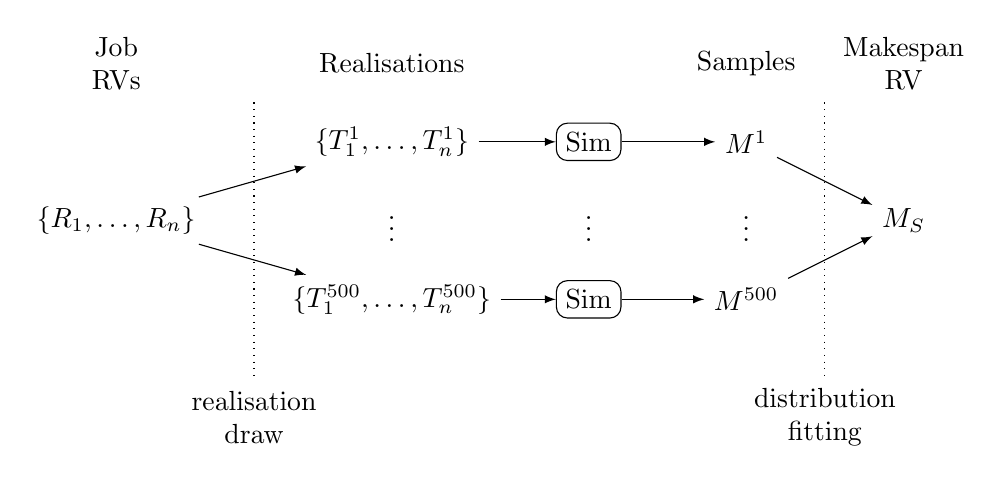
\begin{tikzpicture}[
sim/.style={%
draw, 
rounded corners
}
]
%% Origin node
\node[align=center]at(0,2){Job\\RVs};
\node at(0,0)(orig){$\{R_1,\ldots,R_n\}$};
%% Realisations
\node at(3.5,2){Realisations};
\node[]at(3.5,1)(pert1){$\{T_1^1,\ldots,T_n^1\}$};
\node at(3.5,0){\vdots};
\node at(3.5,-1)(pert5){$\{T_1^{500},\ldots,T_n^{500}\}$};
\draw[-{latex}](orig)--(pert1);
\draw[-{latex}](orig)--(pert5);
%%
\node[sim]at(6,1)(s1){Sim};
\node[sim]at(6,-1)(s5){Sim};
\node at(6,0){\vdots};
\draw[-{latex}](pert1)--(s1);
\draw[-{latex}](pert5)--(s5);
%% Makespans
\node at(8,2){Samples};
\node at(8,1)(M1){$M^1$};
\node at(8,-1)(M5){$M^{500}$};
\node at(8,-0){\vdots};
\draw[-{latex}](s1)--(M1);
\draw[-{latex}](s5)--(M5);
%% Consolidation
\node[align=center]at(10,2){Makespan\\RV};
\node at(10,0)(r){$M_S$};
\draw[-{latex}](M1)--(r);
\draw[-{latex}](M5)--(r);
%%phases
\node[align=center]at(1.75,-2.5)(df){realisation\\draw};
\draw[dotted](1.75,1.5)--(1.75,-2);
\node[align=center]at(9,-2.5)(df){distribution\\fitting};
\draw[dotted](9,1.5)--(9,-2);
\end{tikzpicture}

		}
	\caption{Overview of the Monte-Carlo process : $500$ realisations are
	generated by drawing and adding a perturbation to each job of the
	user provided set, every simulation is then simulated, the resulting
	makespans are fitted into the final result. \label{fig:mcprocess}}
\end{figure}
Fitting is done to a normal distribution because, in essence the makespan is the
sum  of the  runtimes of  the jobs  in the  critical path  of the  schedule.  To
measure the impact  of the runtime perturbation on the  makespan, we compute the
range $[\mu-2\sigma;\mu+2\sigma]$ (that is  a 95\% confidence interval) relative
to  the mean  $\mu$. 
% plus tard, on ? : For  comparison  purpose we  test this  process with  both
%strategies. 
We now  seek to answer the  following two questions: given  a \emph{perturbation
  level}  of  the input  runtimes,  i)  what is  the  convergence  speed of  the
Monte-Carlo  simulation and  ii) what  is the  size of  the confidence  interval
resulting from the Monte-Carlo simulation.

To run  this Monte-Carlo simulation, we  used as user provided runtimes six 
base sets of runtimes obtained by running a Montage\cite{montage2009} workflow.
We call \emph{realisation} a set  of perturbed runtimes. A \emph{realisation} is
based on  a given  base set. For  each job  runtime in the  base set  a separate
relative  perturbation is  drawn  uniformly between  $[1-P,1+P]$,  with $P$  the
perturbation level, and applied to it's given job runtime. For every base set we
generate  500 realisations,  each realisation  receives an  order number.   Every
realisation is then simulated by SimSchlouder.  In order to study the properties
like  convergence  speed  we  opted  to keep  the  results  of  each  individual
simulation indexed  by base set,  perturbation level, and order  number.  Normal
distribution is fitted to data using the maximum likelihood method.

This process was repeated at 4 different perturbation levels, \pmpc{5},
\pmpc{10}, \pmpc{15} and, \pmpc{20}.

\subsection{Monte Carlo Convergence}

Since Monte Carlo methods are based on on repetition of random processes, it is
necessary to repeat the processes enough to obtain the intended result. In
simple Monte Carlo experiments, like integration, the relative error is capped
by $\frac{1}{\sqrt{n}}$ where n is the number of sample, but complex application
can require more more sample or a more targeted sampling to yield correct
results. Our experiment includes both a non trivial simulation step, where
scheduling and job dependency affects which run times are significant, and a
strong aggregation step using normal law fitting fitting. To determine the
convergence properties of our Monte Carlo simulations we observe the evolution
of the normal distribution obtained depending on the number of simulation done. 
Using the simulations order index we are able to produce the fitting we would
had obtained after any arbitrary number of simulation. For every subset we
observe the absolute relative error in the resulting values of $\mu$ and $\sigma$ 
when compared to the value taken when all 500 simulation results are used. 

Table~\ref{tab:mcs-convergence} how many simulations are required before the
absolute error consistently passes under the $.5\%$ threshold average makespan
value $\mu$ and the $1\%$ threshold of the quarter length of the confidence
interval $\sigma$ for different input perturbation levels. For the fitting
process to bear any value we started using at least 5 simulations. The result
show that for this type of simulations at reasonable level of perturbation $\mu$
converges quickly. A hundred simulation is generally enough to get a sense of
the workload makespan. On the other hand the computation of $\sigma$ is much
more volatile and does not appear to exhibit  as strong a convergence. This is
partly compensated by the fact the values of $\sigma$ small compared to the
values of $\mu$.

\begin{table}
	\centering
	%\caption{Monte Carlo simulation convergence based on perturbation}
	\begin{tabular}{rcc|cc|cc|cc}
		\cline{2-9}
		& \multicolumn{2}{c|}{$5\%$}& \multicolumn{2}{c|}{$10\%$}&
		\multicolumn{2}{c|}{$15\%$}& \multicolumn{2}{c}{$20\%$}\\
		&\rot{$\mu.ae<.5\%$}&\rot{$\sigma.ae<1\%$}&\rot{$\mu.ae<.5\%$}&\rot{$\sigma.ae<1\%$}&\rot{$\mu.ae<.5\%$}&\rot{$\sigma.ae<1\%$}&\rot{$\mu.ae<.5\%$}&\rot{$\sigma.ae<1\%$}\\
		\hline
		min&$>5$&$402$&$>5$&$423$&$>5$&$318$&$>5$&$353$\\
		mean&$14$&$448$&$30$&$465$&$29$&$409$&$73$&$442$\\
		max&$44$&$498$&$88$&$490$&$71$&$480$&$238$&$497$\\
		\hline
	\end{tabular}
	\caption{Monte Carlo simulation convergence}
	\label{tab:mcs-convergence}
\end{table}

\subsection{Monte Carlo fitting process}

The fitting process used to aggregate the final result of the Monte Carlo
simulation also possesses it's own confidence characteristic. The method we used
gives a standard deviation for the fitted value of $\mu$ and $\sigma$. Relative
standard deviation as a function of the number of the simulations are shown
figure~\ref{fig:confidence}

\begin{figure}
	\centering
	\resizebox{0.5\textwidth}{!}{%
		% Created by tikzDevice version 0.10.1 on 2017-04-25 14:11:18
% !TEX encoding = UTF-8 Unicode
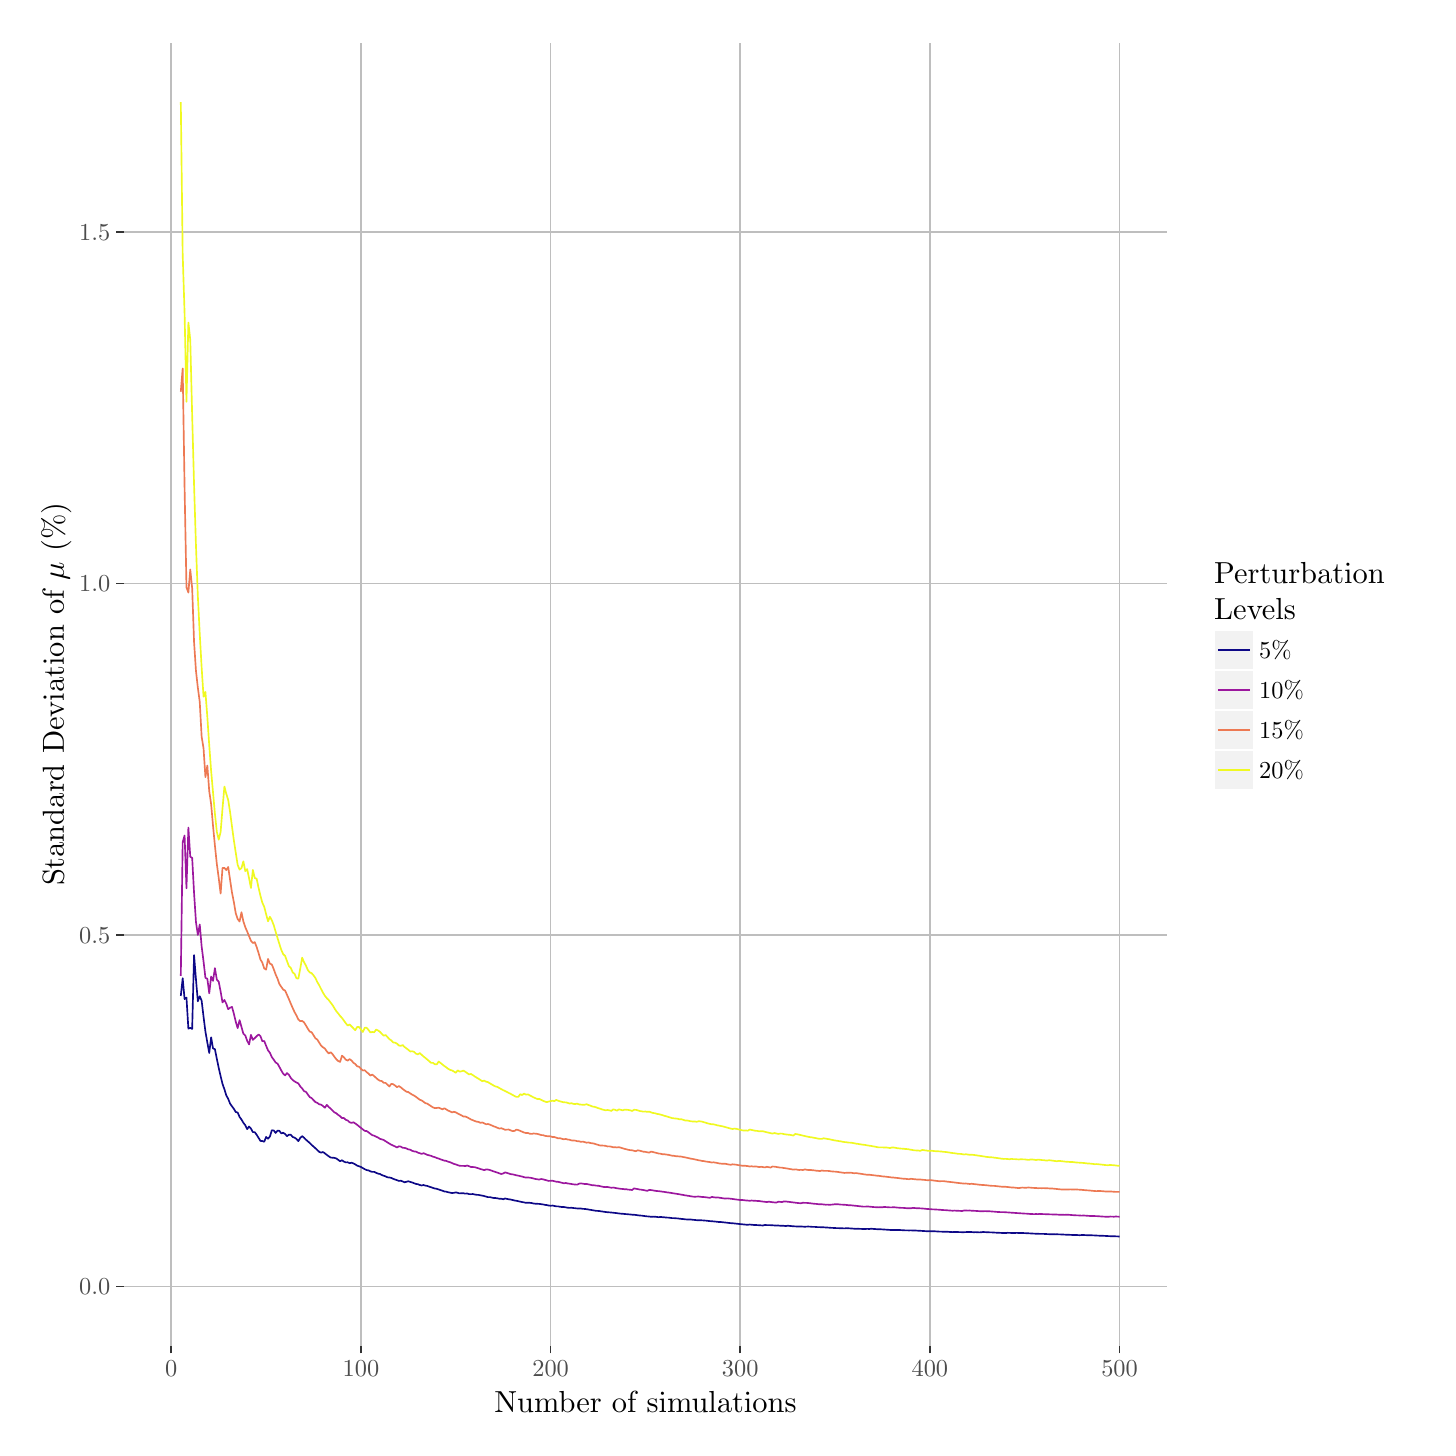
\begin{tikzpicture}[x=1pt,y=1pt]
\definecolor{fillColor}{RGB}{255,255,255}
\path[use as bounding box,fill=fillColor,fill opacity=0.00] (0,0) rectangle (505.89,505.89);
\begin{scope}
\path[clip] (  0.00,  0.00) rectangle (505.89,505.89);
\definecolor{drawColor}{RGB}{255,255,255}
\definecolor{fillColor}{RGB}{255,255,255}

\path[draw=drawColor,line width= 0.6pt,line join=round,line cap=round,fill=fillColor] (  0.00,  0.00) rectangle (505.89,505.89);
\end{scope}
\begin{scope}
\path[clip] ( 34.77, 29.59) rectangle (411.67,500.39);
\definecolor{drawColor}{RGB}{190,190,190}

\path[draw=drawColor,line width= 0.6pt,line join=round] ( 34.77, 50.99) --
	(411.67, 50.99);

\path[draw=drawColor,line width= 0.6pt,line join=round] ( 34.77,178.01) --
	(411.67,178.01);

\path[draw=drawColor,line width= 0.6pt,line join=round] ( 34.77,305.02) --
	(411.67,305.02);

\path[draw=drawColor,line width= 0.6pt,line join=round] ( 34.77,432.04) --
	(411.67,432.04);

\path[draw=drawColor,line width= 0.6pt,line join=round] ( 51.90, 29.59) --
	( 51.90,500.39);

\path[draw=drawColor,line width= 0.6pt,line join=round] (120.43, 29.59) --
	(120.43,500.39);

\path[draw=drawColor,line width= 0.6pt,line join=round] (188.96, 29.59) --
	(188.96,500.39);

\path[draw=drawColor,line width= 0.6pt,line join=round] (257.49, 29.59) --
	(257.49,500.39);

\path[draw=drawColor,line width= 0.6pt,line join=round] (326.01, 29.59) --
	(326.01,500.39);

\path[draw=drawColor,line width= 0.6pt,line join=round] (394.54, 29.59) --
	(394.54,500.39);
\definecolor{drawColor}{RGB}{13,8,135}

\path[draw=drawColor,line width= 0.6pt,line join=round] ( 55.33,156.00) --
	( 56.01,162.39) --
	( 56.70,154.88) --
	( 57.38,155.40) --
	( 58.07,144.17) --
	( 58.75,144.48) --
	( 59.44,144.08) --
	( 60.12,170.76) --
	( 60.81,162.01) --
	( 61.49,154.09) --
	( 62.18,155.89) --
	( 62.86,154.30) --
	( 63.55,148.48) --
	( 64.23,143.13) --
	( 64.92,139.19) --
	( 65.61,135.40) --
	( 66.29,141.05) --
	( 66.98,137.02) --
	( 67.66,136.79) --
	( 68.35,133.29) --
	( 69.03,130.04) --
	( 69.72,127.01) --
	( 70.40,124.23) --
	( 71.09,122.28) --
	( 71.77,120.08) --
	( 72.46,118.81) --
	( 73.14,117.10) --
	( 73.83,116.11) --
	( 74.51,115.20) --
	( 75.20,114.04) --
	( 75.88,113.87) --
	( 76.57,112.29) --
	( 77.26,111.34) --
	( 77.94,110.18) --
	( 78.63,109.29) --
	( 79.31,107.87) --
	( 80.00,108.83) --
	( 80.68,108.07) --
	( 81.37,106.82) --
	( 82.05,106.78) --
	( 82.74,105.84) --
	( 83.42,104.75) --
	( 84.11,103.62) --
	( 84.79,103.57) --
	( 85.48,103.32) --
	( 86.16,105.06) --
	( 86.85,104.42) --
	( 87.53,105.19) --
	( 88.22,107.45) --
	( 88.91,107.42) --
	( 89.59,106.49) --
	( 90.28,107.32) --
	( 90.96,107.26) --
	( 91.65,106.33) --
	( 92.33,106.58) --
	( 93.02,106.11) --
	( 93.70,105.33) --
	( 94.39,105.87) --
	( 95.07,105.86) --
	( 95.76,105.04) --
	( 96.44,104.80) --
	( 97.13,104.32) --
	( 97.81,103.54) --
	( 98.50,104.73) --
	( 99.18,105.35) --
	( 99.87,104.77) --
	(100.56,104.06) --
	(101.24,103.47) --
	(101.93,102.86) --
	(102.61,102.16) --
	(103.30,101.57) --
	(103.98,100.96) --
	(104.67,100.31) --
	(105.35, 99.67) --
	(106.04, 99.37) --
	(106.72, 99.61) --
	(107.41, 99.11) --
	(108.09, 98.58) --
	(108.78, 98.07) --
	(109.46, 97.62) --
	(110.15, 97.54) --
	(110.83, 97.50) --
	(111.52, 97.28) --
	(112.20, 96.78) --
	(112.89, 96.29) --
	(113.58, 96.64) --
	(114.26, 96.16) --
	(114.95, 95.85) --
	(115.63, 95.90) --
	(116.32, 95.56) --
	(117.00, 95.73) --
	(117.69, 95.51) --
	(118.37, 95.13) --
	(119.06, 94.69) --
	(119.74, 94.45) --
	(120.43, 94.20) --
	(121.11, 93.80) --
	(121.80, 93.40) --
	(122.48, 93.07) --
	(123.17, 92.98) --
	(123.85, 92.61) --
	(124.54, 92.42) --
	(125.23, 92.42) --
	(125.91, 92.09) --
	(126.60, 91.80) --
	(127.28, 91.67) --
	(127.97, 91.30) --
	(128.65, 91.03) --
	(129.34, 90.79) --
	(130.02, 90.47) --
	(130.71, 90.39) --
	(131.39, 90.26) --
	(132.08, 89.92) --
	(132.76, 89.67) --
	(133.45, 89.45) --
	(134.13, 89.15) --
	(134.82, 89.24) --
	(135.50, 88.98) --
	(136.19, 88.67) --
	(136.88, 88.86) --
	(137.56, 89.04) --
	(138.25, 88.79) --
	(138.93, 88.62) --
	(139.62, 88.33) --
	(140.30, 88.07) --
	(140.99, 87.98) --
	(141.67, 87.70) --
	(142.36, 87.52) --
	(143.04, 87.68) --
	(143.73, 87.46) --
	(144.41, 87.35) --
	(145.10, 87.08) --
	(145.78, 86.88) --
	(146.47, 86.62) --
	(147.15, 86.41) --
	(147.84, 86.31) --
	(148.52, 86.07) --
	(149.21, 85.84) --
	(149.90, 85.60) --
	(150.58, 85.36) --
	(151.27, 85.27) --
	(151.95, 85.07) --
	(152.64, 84.93) --
	(153.32, 84.79) --
	(154.01, 84.85) --
	(154.69, 85.02) --
	(155.38, 84.87) --
	(156.06, 84.65) --
	(156.75, 84.71) --
	(157.43, 84.72) --
	(158.12, 84.56) --
	(158.80, 84.62) --
	(159.49, 84.41) --
	(160.17, 84.37) --
	(160.86, 84.43) --
	(161.55, 84.26) --
	(162.23, 84.14) --
	(162.92, 84.11) --
	(163.60, 83.96) --
	(164.29, 83.85) --
	(164.97, 83.69) --
	(165.66, 83.49) --
	(166.34, 83.29) --
	(167.03, 83.32) --
	(167.71, 83.15) --
	(168.40, 83.00) --
	(169.08, 82.97) --
	(169.77, 82.88) --
	(170.45, 82.71) --
	(171.14, 82.71) --
	(171.82, 82.54) --
	(172.51, 82.81) --
	(173.20, 82.66) --
	(173.88, 82.53) --
	(174.57, 82.42) --
	(175.25, 82.26) --
	(175.94, 82.09) --
	(176.62, 81.98) --
	(177.31, 81.82) --
	(177.99, 81.68) --
	(178.68, 81.52) --
	(179.36, 81.40) --
	(180.05, 81.25) --
	(180.73, 81.25) --
	(181.42, 81.25) --
	(182.10, 81.17) --
	(182.79, 81.01) --
	(183.47, 80.92) --
	(184.16, 80.89) --
	(184.84, 80.87) --
	(185.53, 80.76) --
	(186.22, 80.66) --
	(186.90, 80.52) --
	(187.59, 80.43) --
	(188.27, 80.28) --
	(188.96, 80.19) --
	(189.64, 80.26) --
	(190.33, 80.11) --
	(191.01, 79.98) --
	(191.70, 79.96) --
	(192.38, 79.82) --
	(193.07, 79.72) --
	(193.75, 79.74) --
	(194.44, 79.61) --
	(195.12, 79.48) --
	(195.81, 79.41) --
	(196.49, 79.47) --
	(197.18, 79.37) --
	(197.87, 79.30) --
	(198.55, 79.21) --
	(199.24, 79.18) --
	(199.92, 79.19) --
	(200.61, 79.06) --
	(201.29, 79.04) --
	(201.98, 78.95) --
	(202.66, 78.83) --
	(203.35, 78.71) --
	(204.03, 78.60) --
	(204.72, 78.47) --
	(205.40, 78.36) --
	(206.09, 78.32) --
	(206.77, 78.25) --
	(207.46, 78.13) --
	(208.14, 78.04) --
	(208.83, 77.93) --
	(209.52, 77.86) --
	(210.20, 77.80) --
	(210.89, 77.75) --
	(211.57, 77.67) --
	(212.26, 77.59) --
	(212.94, 77.52) --
	(213.63, 77.41) --
	(214.31, 77.33) --
	(215.00, 77.30) --
	(215.68, 77.21) --
	(216.37, 77.16) --
	(217.05, 77.10) --
	(217.74, 77.04) --
	(218.42, 76.96) --
	(219.11, 76.94) --
	(219.79, 76.85) --
	(220.48, 76.75) --
	(221.17, 76.66) --
	(221.85, 76.62) --
	(222.54, 76.53) --
	(223.22, 76.43) --
	(223.91, 76.35) --
	(224.59, 76.29) --
	(225.28, 76.20) --
	(225.96, 76.25) --
	(226.65, 76.22) --
	(227.33, 76.15) --
	(228.02, 76.06) --
	(228.70, 76.15) --
	(229.39, 76.06) --
	(230.07, 76.01) --
	(230.76, 75.92) --
	(231.44, 75.91) --
	(232.13, 75.82) --
	(232.81, 75.73) --
	(233.50, 75.72) --
	(234.19, 75.66) --
	(234.87, 75.61) --
	(235.56, 75.52) --
	(236.24, 75.43) --
	(236.93, 75.37) --
	(237.61, 75.29) --
	(238.30, 75.22) --
	(238.98, 75.23) --
	(239.67, 75.21) --
	(240.35, 75.12) --
	(241.04, 75.06) --
	(241.72, 74.98) --
	(242.41, 74.94) --
	(243.09, 74.95) --
	(243.78, 74.91) --
	(244.46, 74.86) --
	(245.15, 74.80) --
	(245.84, 74.72) --
	(246.52, 74.64) --
	(247.21, 74.59) --
	(247.89, 74.53) --
	(248.58, 74.46) --
	(249.26, 74.38) --
	(249.95, 74.30) --
	(250.63, 74.29) --
	(251.32, 74.21) --
	(252.00, 74.14) --
	(252.69, 74.06) --
	(253.37, 73.98) --
	(254.06, 73.90) --
	(254.74, 73.86) --
	(255.43, 73.79) --
	(256.11, 73.71) --
	(256.80, 73.64) --
	(257.49, 73.56) --
	(258.17, 73.49) --
	(258.86, 73.42) --
	(259.54, 73.35) --
	(260.23, 73.32) --
	(260.91, 73.40) --
	(261.60, 73.33) --
	(262.28, 73.26) --
	(262.97, 73.26) --
	(263.65, 73.19) --
	(264.34, 73.16) --
	(265.02, 73.11) --
	(265.71, 73.05) --
	(266.39, 73.26) --
	(267.08, 73.19) --
	(267.76, 73.19) --
	(268.45, 73.17) --
	(269.13, 73.13) --
	(269.82, 73.08) --
	(270.51, 73.02) --
	(271.19, 73.05) --
	(271.88, 72.98) --
	(272.56, 72.99) --
	(273.25, 72.93) --
	(273.93, 72.86) --
	(274.62, 72.97) --
	(275.30, 72.91) --
	(275.99, 72.84) --
	(276.67, 72.77) --
	(277.36, 72.74) --
	(278.04, 72.69) --
	(278.73, 72.67) --
	(279.41, 72.68) --
	(280.10, 72.66) --
	(280.78, 72.59) --
	(281.47, 72.66) --
	(282.16, 72.67) --
	(282.84, 72.63) --
	(283.53, 72.56) --
	(284.21, 72.56) --
	(284.90, 72.52) --
	(285.58, 72.45) --
	(286.27, 72.46) --
	(286.95, 72.41) --
	(287.64, 72.40) --
	(288.32, 72.35) --
	(289.01, 72.31) --
	(289.69, 72.26) --
	(290.38, 72.20) --
	(291.06, 72.18) --
	(291.75, 72.13) --
	(292.43, 72.11) --
	(293.12, 72.09) --
	(293.81, 72.03) --
	(294.49, 72.04) --
	(295.18, 72.00) --
	(295.86, 72.10) --
	(296.55, 72.05) --
	(297.23, 72.00) --
	(297.92, 71.95) --
	(298.60, 71.90) --
	(299.29, 71.84) --
	(299.97, 71.89) --
	(300.66, 71.84) --
	(301.34, 71.82) --
	(302.03, 71.77) --
	(302.71, 71.80) --
	(303.40, 71.84) --
	(304.08, 71.79) --
	(304.77, 71.88) --
	(305.46, 71.83) --
	(306.14, 71.78) --
	(306.83, 71.72) --
	(307.51, 71.67) --
	(308.20, 71.69) --
	(308.88, 71.64) --
	(309.57, 71.60) --
	(310.25, 71.55) --
	(310.94, 71.50) --
	(311.62, 71.45) --
	(312.31, 71.44) --
	(312.99, 71.43) --
	(313.68, 71.45) --
	(314.36, 71.42) --
	(315.05, 71.42) --
	(315.73, 71.38) --
	(316.42, 71.34) --
	(317.10, 71.29) --
	(317.79, 71.29) --
	(318.48, 71.27) --
	(319.16, 71.29) --
	(319.85, 71.25) --
	(320.53, 71.26) --
	(321.22, 71.21) --
	(321.90, 71.16) --
	(322.59, 71.14) --
	(323.27, 71.09) --
	(323.96, 71.05) --
	(324.64, 71.00) --
	(325.33, 70.97) --
	(326.01, 71.01) --
	(326.70, 70.97) --
	(327.38, 70.98) --
	(328.07, 70.94) --
	(328.75, 70.89) --
	(329.44, 70.85) --
	(330.13, 70.83) --
	(330.81, 70.81) --
	(331.50, 70.82) --
	(332.18, 70.80) --
	(332.87, 70.75) --
	(333.55, 70.70) --
	(334.24, 70.67) --
	(334.92, 70.70) --
	(335.61, 70.70) --
	(336.29, 70.68) --
	(336.98, 70.65) --
	(337.66, 70.64) --
	(338.35, 70.64) --
	(339.03, 70.67) --
	(339.72, 70.73) --
	(340.40, 70.70) --
	(341.09, 70.68) --
	(341.78, 70.63) --
	(342.46, 70.65) --
	(343.15, 70.62) --
	(343.83, 70.57) --
	(344.52, 70.61) --
	(345.20, 70.71) --
	(345.89, 70.66) --
	(346.57, 70.63) --
	(347.26, 70.59) --
	(347.94, 70.58) --
	(348.63, 70.55) --
	(349.31, 70.50) --
	(350.00, 70.46) --
	(350.68, 70.42) --
	(351.37, 70.40) --
	(352.05, 70.36) --
	(352.74, 70.32) --
	(353.42, 70.33) --
	(354.11, 70.41) --
	(354.80, 70.39) --
	(355.48, 70.36) --
	(356.17, 70.36) --
	(356.85, 70.37) --
	(357.54, 70.38) --
	(358.22, 70.35) --
	(358.91, 70.34) --
	(359.59, 70.33) --
	(360.28, 70.30) --
	(360.96, 70.26) --
	(361.65, 70.23) --
	(362.33, 70.19) --
	(363.02, 70.15) --
	(363.70, 70.11) --
	(364.39, 70.09) --
	(365.07, 70.05) --
	(365.76, 70.04) --
	(366.45, 70.04) --
	(367.13, 70.02) --
	(367.82, 69.99) --
	(368.50, 69.94) --
	(369.19, 69.91) --
	(369.87, 69.88) --
	(370.56, 69.90) --
	(371.24, 69.86) --
	(371.93, 69.88) --
	(372.61, 69.85) --
	(373.30, 69.83) --
	(373.98, 69.80) --
	(374.67, 69.76) --
	(375.35, 69.72) --
	(376.04, 69.69) --
	(376.72, 69.68) --
	(377.41, 69.64) --
	(378.10, 69.62) --
	(378.78, 69.62) --
	(379.47, 69.59) --
	(380.15, 69.55) --
	(380.84, 69.61) --
	(381.52, 69.61) --
	(382.21, 69.58) --
	(382.89, 69.54) --
	(383.58, 69.55) --
	(384.26, 69.52) --
	(384.95, 69.49) --
	(385.63, 69.46) --
	(386.32, 69.42) --
	(387.00, 69.38) --
	(387.69, 69.37) --
	(388.37, 69.34) --
	(389.06, 69.31) --
	(389.75, 69.27) --
	(390.43, 69.23) --
	(391.12, 69.20) --
	(391.80, 69.18) --
	(392.49, 69.18) --
	(393.17, 69.14) --
	(393.86, 69.11) --
	(394.54, 69.08);
\definecolor{drawColor}{RGB}{156,23,158}

\path[draw=drawColor,line width= 0.6pt,line join=round] ( 55.33,163.25) --
	( 56.01,211.53) --
	( 56.70,213.97) --
	( 57.38,194.92) --
	( 58.07,216.87) --
	( 58.75,206.30) --
	( 59.44,205.89) --
	( 60.12,193.27) --
	( 60.81,182.74) --
	( 61.49,178.04) --
	( 62.18,181.83) --
	( 62.86,173.93) --
	( 63.55,168.47) --
	( 64.23,162.55) --
	( 64.92,162.22) --
	( 65.61,156.94) --
	( 66.29,163.01) --
	( 66.98,161.47) --
	( 67.66,166.05) --
	( 68.35,161.89) --
	( 69.03,161.16) --
	( 69.72,157.61) --
	( 70.40,153.68) --
	( 71.09,154.55) --
	( 71.77,153.19) --
	( 72.46,151.22) --
	( 73.14,151.74) --
	( 73.83,152.04) --
	( 74.51,149.56) --
	( 75.20,146.66) --
	( 75.88,144.37) --
	( 76.57,147.27) --
	( 77.26,144.78) --
	( 77.94,142.35) --
	( 78.63,141.73) --
	( 79.31,139.82) --
	( 80.00,138.47) --
	( 80.68,141.94) --
	( 81.37,140.14) --
	( 82.05,140.75) --
	( 82.74,141.45) --
	( 83.42,142.09) --
	( 84.11,141.48) --
	( 84.79,139.66) --
	( 85.48,139.71) --
	( 86.16,137.99) --
	( 86.85,136.35) --
	( 87.53,135.47) --
	( 88.22,133.90) --
	( 88.91,132.99) --
	( 89.59,131.96) --
	( 90.28,131.54) --
	( 90.96,130.35) --
	( 91.65,129.05) --
	( 92.33,127.91) --
	( 93.02,127.30) --
	( 93.70,128.12) --
	( 94.39,127.54) --
	( 95.07,126.38) --
	( 95.76,125.64) --
	( 96.44,125.12) --
	( 97.13,124.71) --
	( 97.81,124.38) --
	( 98.50,123.31) --
	( 99.18,122.59) --
	( 99.87,121.59) --
	(100.56,121.35) --
	(101.24,120.39) --
	(101.93,119.44) --
	(102.61,119.10) --
	(103.30,118.34) --
	(103.98,117.65) --
	(104.67,117.36) --
	(105.35,116.84) --
	(106.04,116.72) --
	(106.72,116.22) --
	(107.41,115.61) --
	(108.09,116.64) --
	(108.78,115.89) --
	(109.46,115.30) --
	(110.15,114.60) --
	(110.83,113.95) --
	(111.52,113.61) --
	(112.20,113.01) --
	(112.89,112.55) --
	(113.58,111.87) --
	(114.26,111.88) --
	(114.95,111.24) --
	(115.63,111.01) --
	(116.32,110.37) --
	(117.00,110.12) --
	(117.69,110.36) --
	(118.37,109.94) --
	(119.06,109.43) --
	(119.74,108.86) --
	(120.43,108.33) --
	(121.11,107.78) --
	(121.80,107.24) --
	(122.48,107.18) --
	(123.17,106.71) --
	(123.85,106.18) --
	(124.54,105.67) --
	(125.23,105.51) --
	(125.91,105.15) --
	(126.60,104.84) --
	(127.28,104.36) --
	(127.97,104.18) --
	(128.65,103.95) --
	(129.34,103.50) --
	(130.02,103.07) --
	(130.71,102.65) --
	(131.39,102.24) --
	(132.08,101.94) --
	(132.76,101.62) --
	(133.45,101.23) --
	(134.13,101.68) --
	(134.82,101.55) --
	(135.50,101.14) --
	(136.19,101.09) --
	(136.88,100.90) --
	(137.56,100.56) --
	(138.25,100.43) --
	(138.93,100.04) --
	(139.62, 99.83) --
	(140.30, 99.75) --
	(140.99, 99.39) --
	(141.67, 99.18) --
	(142.36, 98.91) --
	(143.04, 99.18) --
	(143.73, 98.88) --
	(144.41, 98.58) --
	(145.10, 98.41) --
	(145.78, 98.22) --
	(146.47, 97.92) --
	(147.15, 97.75) --
	(147.84, 97.42) --
	(148.52, 97.24) --
	(149.21, 96.96) --
	(149.90, 96.73) --
	(150.58, 96.48) --
	(151.27, 96.40) --
	(151.95, 96.10) --
	(152.64, 95.92) --
	(153.32, 95.62) --
	(154.01, 95.32) --
	(154.69, 95.12) --
	(155.38, 94.87) --
	(156.06, 94.64) --
	(156.75, 94.59) --
	(157.43, 94.61) --
	(158.12, 94.52) --
	(158.80, 94.73) --
	(159.49, 94.48) --
	(160.17, 94.20) --
	(160.86, 94.18) --
	(161.55, 94.13) --
	(162.23, 93.91) --
	(162.92, 93.72) --
	(163.60, 93.46) --
	(164.29, 93.28) --
	(164.97, 93.04) --
	(165.66, 93.34) --
	(166.34, 93.27) --
	(167.03, 93.10) --
	(167.71, 92.85) --
	(168.40, 92.61) --
	(169.08, 92.37) --
	(169.77, 92.14) --
	(170.45, 91.90) --
	(171.14, 91.67) --
	(171.82, 91.86) --
	(172.51, 92.23) --
	(173.20, 92.06) --
	(173.88, 91.83) --
	(174.57, 91.61) --
	(175.25, 91.53) --
	(175.94, 91.36) --
	(176.62, 91.18) --
	(177.31, 91.06) --
	(177.99, 90.89) --
	(178.68, 90.74) --
	(179.36, 90.52) --
	(180.05, 90.38) --
	(180.73, 90.42) --
	(181.42, 90.33) --
	(182.10, 90.22) --
	(182.79, 90.04) --
	(183.47, 89.87) --
	(184.16, 89.75) --
	(184.84, 89.66) --
	(185.53, 89.85) --
	(186.22, 89.74) --
	(186.90, 89.54) --
	(187.59, 89.36) --
	(188.27, 89.16) --
	(188.96, 89.21) --
	(189.64, 89.23) --
	(190.33, 89.05) --
	(191.01, 88.89) --
	(191.70, 88.84) --
	(192.38, 88.66) --
	(193.07, 88.48) --
	(193.75, 88.31) --
	(194.44, 88.42) --
	(195.12, 88.25) --
	(195.81, 88.16) --
	(196.49, 88.05) --
	(197.18, 87.93) --
	(197.87, 87.86) --
	(198.55, 87.81) --
	(199.24, 88.17) --
	(199.92, 88.29) --
	(200.61, 88.15) --
	(201.29, 88.04) --
	(201.98, 88.08) --
	(202.66, 87.92) --
	(203.35, 87.76) --
	(204.03, 87.59) --
	(204.72, 87.58) --
	(205.40, 87.45) --
	(206.09, 87.44) --
	(206.77, 87.29) --
	(207.46, 87.13) --
	(208.14, 86.98) --
	(208.83, 86.93) --
	(209.52, 86.97) --
	(210.20, 86.83) --
	(210.89, 86.69) --
	(211.57, 86.77) --
	(212.26, 86.65) --
	(212.94, 86.50) --
	(213.63, 86.40) --
	(214.31, 86.30) --
	(215.00, 86.25) --
	(215.68, 86.17) --
	(216.37, 86.15) --
	(217.05, 86.01) --
	(217.74, 85.99) --
	(218.42, 85.87) --
	(219.11, 86.46) --
	(219.79, 86.32) --
	(220.48, 86.19) --
	(221.17, 86.05) --
	(221.85, 85.98) --
	(222.54, 85.85) --
	(223.22, 85.71) --
	(223.91, 85.57) --
	(224.59, 85.90) --
	(225.28, 85.85) --
	(225.96, 85.74) --
	(226.65, 85.61) --
	(227.33, 85.51) --
	(228.02, 85.46) --
	(228.70, 85.38) --
	(229.39, 85.27) --
	(230.07, 85.19) --
	(230.76, 85.06) --
	(231.44, 84.98) --
	(232.13, 84.89) --
	(232.81, 84.77) --
	(233.50, 84.65) --
	(234.19, 84.55) --
	(234.87, 84.44) --
	(235.56, 84.32) --
	(236.24, 84.20) --
	(236.93, 84.08) --
	(237.61, 83.95) --
	(238.30, 83.84) --
	(238.98, 83.73) --
	(239.67, 83.61) --
	(240.35, 83.49) --
	(241.04, 83.45) --
	(241.72, 83.48) --
	(242.41, 83.54) --
	(243.09, 83.43) --
	(243.78, 83.35) --
	(244.46, 83.32) --
	(245.15, 83.25) --
	(245.84, 83.15) --
	(246.52, 83.05) --
	(247.21, 83.37) --
	(247.89, 83.27) --
	(248.58, 83.16) --
	(249.26, 83.21) --
	(249.95, 83.10) --
	(250.63, 82.99) --
	(251.32, 82.88) --
	(252.00, 82.78) --
	(252.69, 82.86) --
	(253.37, 82.80) --
	(254.06, 82.73) --
	(254.74, 82.64) --
	(255.43, 82.53) --
	(256.11, 82.44) --
	(256.80, 82.36) --
	(257.49, 82.25) --
	(258.17, 82.29) --
	(258.86, 82.19) --
	(259.54, 82.11) --
	(260.23, 82.06) --
	(260.91, 81.98) --
	(261.60, 82.08) --
	(262.28, 82.00) --
	(262.97, 81.98) --
	(263.65, 81.92) --
	(264.34, 81.89) --
	(265.02, 81.79) --
	(265.71, 81.69) --
	(266.39, 81.61) --
	(267.08, 81.52) --
	(267.76, 81.65) --
	(268.45, 81.57) --
	(269.13, 81.47) --
	(269.82, 81.40) --
	(270.51, 81.32) --
	(271.19, 81.63) --
	(271.88, 81.60) --
	(272.56, 81.52) --
	(273.25, 81.76) --
	(273.93, 81.73) --
	(274.62, 81.64) --
	(275.30, 81.57) --
	(275.99, 81.47) --
	(276.67, 81.39) --
	(277.36, 81.30) --
	(278.04, 81.21) --
	(278.73, 81.14) --
	(279.41, 81.09) --
	(280.10, 81.27) --
	(280.78, 81.23) --
	(281.47, 81.22) --
	(282.16, 81.16) --
	(282.84, 81.08) --
	(283.53, 80.99) --
	(284.21, 80.90) --
	(284.90, 80.86) --
	(285.58, 80.78) --
	(286.27, 80.71) --
	(286.95, 80.73) --
	(287.64, 80.65) --
	(288.32, 80.57) --
	(289.01, 80.60) --
	(289.69, 80.51) --
	(290.38, 80.59) --
	(291.06, 80.64) --
	(291.75, 80.76) --
	(292.43, 80.76) --
	(293.12, 80.69) --
	(293.81, 80.61) --
	(294.49, 80.58) --
	(295.18, 80.55) --
	(295.86, 80.48) --
	(296.55, 80.39) --
	(297.23, 80.39) --
	(297.92, 80.31) --
	(298.60, 80.23) --
	(299.29, 80.17) --
	(299.97, 80.09) --
	(300.66, 80.01) --
	(301.34, 79.94) --
	(302.03, 79.86) --
	(302.71, 79.87) --
	(303.40, 79.95) --
	(304.08, 79.87) --
	(304.77, 79.81) --
	(305.46, 79.73) --
	(306.14, 79.68) --
	(306.83, 79.67) --
	(307.51, 79.61) --
	(308.20, 79.68) --
	(308.88, 79.64) --
	(309.57, 79.77) --
	(310.25, 79.69) --
	(310.94, 79.66) --
	(311.62, 79.60) --
	(312.31, 79.61) --
	(312.99, 79.67) --
	(313.68, 79.59) --
	(314.36, 79.52) --
	(315.05, 79.48) --
	(315.73, 79.41) --
	(316.42, 79.42) --
	(317.10, 79.35) --
	(317.79, 79.30) --
	(318.48, 79.26) --
	(319.16, 79.27) --
	(319.85, 79.43) --
	(320.53, 79.36) --
	(321.22, 79.30) --
	(321.90, 79.29) --
	(322.59, 79.24) --
	(323.27, 79.21) --
	(323.96, 79.14) --
	(324.64, 79.07) --
	(325.33, 79.00) --
	(326.01, 78.97) --
	(326.70, 78.90) --
	(327.38, 78.88) --
	(328.07, 78.84) --
	(328.75, 78.79) --
	(329.44, 78.76) --
	(330.13, 78.69) --
	(330.81, 78.63) --
	(331.50, 78.61) --
	(332.18, 78.55) --
	(332.87, 78.50) --
	(333.55, 78.45) --
	(334.24, 78.39) --
	(334.92, 78.45) --
	(335.61, 78.38) --
	(336.29, 78.36) --
	(336.98, 78.34) --
	(337.66, 78.27) --
	(338.35, 78.49) --
	(339.03, 78.49) --
	(339.72, 78.43) --
	(340.40, 78.47) --
	(341.09, 78.40) --
	(341.78, 78.36) --
	(342.46, 78.34) --
	(343.15, 78.28) --
	(343.83, 78.24) --
	(344.52, 78.19) --
	(345.20, 78.18) --
	(345.89, 78.26) --
	(346.57, 78.21) --
	(347.26, 78.22) --
	(347.94, 78.16) --
	(348.63, 78.10) --
	(349.31, 78.05) --
	(350.00, 77.99) --
	(350.68, 77.93) --
	(351.37, 77.90) --
	(352.05, 77.88) --
	(352.74, 77.89) --
	(353.42, 77.83) --
	(354.11, 77.79) --
	(354.80, 77.74) --
	(355.48, 77.68) --
	(356.17, 77.64) --
	(356.85, 77.59) --
	(357.54, 77.54) --
	(358.22, 77.50) --
	(358.91, 77.45) --
	(359.59, 77.41) --
	(360.28, 77.36) --
	(360.96, 77.33) --
	(361.65, 77.27) --
	(362.33, 77.22) --
	(363.02, 77.19) --
	(363.70, 77.16) --
	(364.39, 77.20) --
	(365.07, 77.16) --
	(365.76, 77.25) --
	(366.45, 77.19) --
	(367.13, 77.17) --
	(367.82, 77.14) --
	(368.50, 77.11) --
	(369.19, 77.09) --
	(369.87, 77.08) --
	(370.56, 77.02) --
	(371.24, 77.06) --
	(371.93, 77.00) --
	(372.61, 76.96) --
	(373.30, 76.96) --
	(373.98, 76.95) --
	(374.67, 76.90) --
	(375.35, 76.95) --
	(376.04, 76.93) --
	(376.72, 76.88) --
	(377.41, 76.82) --
	(378.10, 76.77) --
	(378.78, 76.73) --
	(379.47, 76.72) --
	(380.15, 76.66) --
	(380.84, 76.62) --
	(381.52, 76.67) --
	(382.21, 76.62) --
	(382.89, 76.57) --
	(383.58, 76.52) --
	(384.26, 76.48) --
	(384.95, 76.47) --
	(385.63, 76.46) --
	(386.32, 76.44) --
	(387.00, 76.39) --
	(387.69, 76.34) --
	(388.37, 76.29) --
	(389.06, 76.25) --
	(389.75, 76.20) --
	(390.43, 76.20) --
	(391.12, 76.28) --
	(391.80, 76.27) --
	(392.49, 76.23) --
	(393.17, 76.30) --
	(393.86, 76.26) --
	(394.54, 76.23);
\definecolor{drawColor}{RGB}{237,121,83}

\path[draw=drawColor,line width= 0.6pt,line join=round] ( 55.33,374.32) --
	( 56.01,382.74) --
	( 56.70,339.63) --
	( 57.38,303.64) --
	( 58.07,301.75) --
	( 58.75,310.07) --
	( 59.44,303.36) --
	( 60.12,283.96) --
	( 60.81,273.46) --
	( 61.49,267.40) --
	( 62.18,262.22) --
	( 62.86,249.73) --
	( 63.55,245.46) --
	( 64.23,235.09) --
	( 64.92,239.25) --
	( 65.61,229.98) --
	( 66.29,225.35) --
	( 66.98,217.43) --
	( 67.66,210.33) --
	( 68.35,203.71) --
	( 69.03,198.66) --
	( 69.72,193.01) --
	( 70.40,202.21) --
	( 71.09,202.27) --
	( 71.77,201.47) --
	( 72.46,202.61) --
	( 73.14,197.93) --
	( 73.83,193.34) --
	( 74.51,189.88) --
	( 75.20,185.80) --
	( 75.88,183.80) --
	( 76.57,182.91) --
	( 77.26,186.24) --
	( 77.94,182.91) --
	( 78.63,180.86) --
	( 79.31,179.29) --
	( 80.00,177.60) --
	( 80.68,175.93) --
	( 81.37,175.13) --
	( 82.05,175.46) --
	( 82.74,173.68) --
	( 83.42,171.55) --
	( 84.11,169.16) --
	( 84.79,168.04) --
	( 85.48,165.93) --
	( 86.16,165.53) --
	( 86.85,169.38) --
	( 87.53,167.67) --
	( 88.22,167.38) --
	( 88.91,165.69) --
	( 89.59,163.81) --
	( 90.28,162.24) --
	( 90.96,160.31) --
	( 91.65,159.29) --
	( 92.33,158.29) --
	( 93.02,157.95) --
	( 93.70,156.42) --
	( 94.39,154.88) --
	( 95.07,153.23) --
	( 95.76,151.65) --
	( 96.44,150.17) --
	( 97.13,148.93) --
	( 97.81,147.50) --
	( 98.50,146.90) --
	( 99.18,146.99) --
	( 99.87,146.44) --
	(100.56,145.33) --
	(101.24,144.18) --
	(101.93,143.11) --
	(102.61,142.89) --
	(103.30,141.80) --
	(103.98,140.69) --
	(104.67,140.22) --
	(105.35,139.12) --
	(106.04,138.05) --
	(106.72,137.43) --
	(107.41,136.99) --
	(108.09,135.98) --
	(108.78,135.23) --
	(109.46,135.67) --
	(110.15,135.00) --
	(110.83,134.03) --
	(111.52,133.13) --
	(112.20,132.49) --
	(112.89,132.17) --
	(113.58,134.41) --
	(114.26,133.85) --
	(114.95,132.96) --
	(115.63,132.64) --
	(116.32,133.17) --
	(117.00,132.71) --
	(117.69,131.86) --
	(118.37,131.41) --
	(119.06,130.59) --
	(119.74,130.43) --
	(120.43,129.66) --
	(121.11,129.07) --
	(121.80,129.16) --
	(122.48,128.46) --
	(123.17,127.94) --
	(123.85,127.22) --
	(124.54,127.58) --
	(125.23,127.00) --
	(125.91,126.39) --
	(126.60,125.78) --
	(127.28,125.35) --
	(127.97,125.26) --
	(128.65,124.60) --
	(129.34,124.57) --
	(130.02,123.93) --
	(130.71,123.30) --
	(131.39,124.23) --
	(132.08,124.11) --
	(132.76,123.63) --
	(133.45,123.02) --
	(134.13,123.45) --
	(134.82,122.98) --
	(135.50,122.40) --
	(136.19,121.89) --
	(136.88,121.39) --
	(137.56,121.27) --
	(138.25,120.77) --
	(138.93,120.34) --
	(139.62,120.00) --
	(140.30,119.54) --
	(140.99,119.02) --
	(141.67,118.51) --
	(142.36,118.25) --
	(143.04,117.76) --
	(143.73,117.26) --
	(144.41,117.09) --
	(145.10,116.61) --
	(145.78,116.15) --
	(146.47,115.73) --
	(147.15,115.46) --
	(147.84,115.53) --
	(148.52,115.62) --
	(149.21,115.33) --
	(149.90,115.05) --
	(150.58,115.41) --
	(151.27,114.99) --
	(151.95,114.57) --
	(152.64,114.30) --
	(153.32,113.92) --
	(154.01,114.15) --
	(154.69,113.94) --
	(155.38,113.54) --
	(156.06,113.21) --
	(156.75,112.85) --
	(157.43,112.45) --
	(158.12,112.43) --
	(158.80,112.15) --
	(159.49,111.77) --
	(160.17,111.38) --
	(160.86,111.10) --
	(161.55,110.81) --
	(162.23,110.57) --
	(162.92,110.50) --
	(163.60,110.16) --
	(164.29,110.28) --
	(164.97,109.95) --
	(165.66,109.65) --
	(166.34,109.73) --
	(167.03,109.51) --
	(167.71,109.20) --
	(168.40,108.89) --
	(169.08,108.68) --
	(169.77,108.35) --
	(170.45,108.09) --
	(171.14,108.21) --
	(171.82,107.95) --
	(172.51,107.63) --
	(173.20,107.71) --
	(173.88,107.72) --
	(174.57,107.41) --
	(175.25,107.15) --
	(175.94,107.24) --
	(176.62,107.72) --
	(177.31,107.52) --
	(177.99,107.24) --
	(178.68,106.94) --
	(179.36,106.66) --
	(180.05,106.47) --
	(180.73,106.51) --
	(181.42,106.22) --
	(182.10,106.15) --
	(182.79,106.29) --
	(183.47,106.24) --
	(184.16,106.16) --
	(184.84,105.97) --
	(185.53,105.73) --
	(186.22,105.72) --
	(186.90,105.45) --
	(187.59,105.35) --
	(188.27,105.30) --
	(188.96,105.27) --
	(189.64,105.01) --
	(190.33,105.01) --
	(191.01,104.79) --
	(191.70,104.53) --
	(192.38,104.62) --
	(193.07,104.37) --
	(193.75,104.21) --
	(194.44,104.35) --
	(195.12,104.12) --
	(195.81,104.04) --
	(196.49,103.80) --
	(197.18,103.77) --
	(197.87,103.72) --
	(198.55,103.53) --
	(199.24,103.48) --
	(199.92,103.26) --
	(200.61,103.38) --
	(201.29,103.18) --
	(201.98,102.97) --
	(202.66,103.06) --
	(203.35,102.86) --
	(204.03,102.76) --
	(204.72,102.64) --
	(205.40,102.41) --
	(206.09,102.19) --
	(206.77,101.99) --
	(207.46,101.95) --
	(208.14,101.92) --
	(208.83,101.84) --
	(209.52,101.62) --
	(210.20,101.66) --
	(210.89,101.52) --
	(211.57,101.30) --
	(212.26,101.34) --
	(212.94,101.26) --
	(213.63,101.37) --
	(214.31,101.17) --
	(215.00,100.96) --
	(215.68,100.75) --
	(216.37,100.59) --
	(217.05,100.40) --
	(217.74,100.28) --
	(218.42,100.24) --
	(219.11,100.04) --
	(219.79, 99.90) --
	(220.48,100.24) --
	(221.17,100.09) --
	(221.85, 99.90) --
	(222.54, 99.70) --
	(223.22, 99.67) --
	(223.91, 99.50) --
	(224.59, 99.38) --
	(225.28, 99.77) --
	(225.96, 99.60) --
	(226.65, 99.41) --
	(227.33, 99.25) --
	(228.02, 99.06) --
	(228.70, 98.99) --
	(229.39, 98.81) --
	(230.07, 98.81) --
	(230.76, 98.69) --
	(231.44, 98.61) --
	(232.13, 98.46) --
	(232.81, 98.28) --
	(233.50, 98.25) --
	(234.19, 98.10) --
	(234.87, 98.06) --
	(235.56, 97.99) --
	(236.24, 97.95) --
	(236.93, 97.78) --
	(237.61, 97.67) --
	(238.30, 97.51) --
	(238.98, 97.36) --
	(239.67, 97.19) --
	(240.35, 97.10) --
	(241.04, 96.95) --
	(241.72, 96.79) --
	(242.41, 96.64) --
	(243.09, 96.52) --
	(243.78, 96.37) --
	(244.46, 96.31) --
	(245.15, 96.15) --
	(245.84, 96.07) --
	(246.52, 95.96) --
	(247.21, 95.83) --
	(247.89, 95.89) --
	(248.58, 95.76) --
	(249.26, 95.62) --
	(249.95, 95.47) --
	(250.63, 95.40) --
	(251.32, 95.35) --
	(252.00, 95.38) --
	(252.69, 95.23) --
	(253.37, 95.10) --
	(254.06, 94.99) --
	(254.74, 95.17) --
	(255.43, 95.09) --
	(256.11, 95.01) --
	(256.80, 94.87) --
	(257.49, 94.78) --
	(258.17, 94.64) --
	(258.86, 94.68) --
	(259.54, 94.60) --
	(260.23, 94.51) --
	(260.91, 94.38) --
	(261.60, 94.46) --
	(262.28, 94.32) --
	(262.97, 94.40) --
	(263.65, 94.30) --
	(264.34, 94.16) --
	(265.02, 94.27) --
	(265.71, 94.17) --
	(266.39, 94.04) --
	(267.08, 94.27) --
	(267.76, 94.14) --
	(268.45, 94.00) --
	(269.13, 94.36) --
	(269.82, 94.32) --
	(270.51, 94.22) --
	(271.19, 94.09) --
	(271.88, 93.98) --
	(272.56, 93.95) --
	(273.25, 93.82) --
	(273.93, 93.74) --
	(274.62, 93.61) --
	(275.30, 93.49) --
	(275.99, 93.37) --
	(276.67, 93.24) --
	(277.36, 93.34) --
	(278.04, 93.24) --
	(278.73, 93.11) --
	(279.41, 93.18) --
	(280.10, 93.09) --
	(280.78, 93.33) --
	(281.47, 93.20) --
	(282.16, 93.09) --
	(282.84, 93.14) --
	(283.53, 93.03) --
	(284.21, 92.98) --
	(284.90, 92.86) --
	(285.58, 92.82) --
	(286.27, 92.70) --
	(286.95, 92.93) --
	(287.64, 92.81) --
	(288.32, 92.78) --
	(289.01, 92.80) --
	(289.69, 92.73) --
	(290.38, 92.62) --
	(291.06, 92.55) --
	(291.75, 92.52) --
	(292.43, 92.46) --
	(293.12, 92.35) --
	(293.81, 92.24) --
	(294.49, 92.15) --
	(295.18, 92.04) --
	(295.86, 92.11) --
	(296.55, 92.11) --
	(297.23, 92.15) --
	(297.92, 92.06) --
	(298.60, 91.94) --
	(299.29, 92.00) --
	(299.97, 91.89) --
	(300.66, 91.79) --
	(301.34, 91.69) --
	(302.03, 91.58) --
	(302.71, 91.47) --
	(303.40, 91.37) --
	(304.08, 91.41) --
	(304.77, 91.31) --
	(305.46, 91.23) --
	(306.14, 91.15) --
	(306.83, 91.05) --
	(307.51, 91.01) --
	(308.20, 90.91) --
	(308.88, 90.80) --
	(309.57, 90.75) --
	(310.25, 90.68) --
	(310.94, 90.58) --
	(311.62, 90.51) --
	(312.31, 90.40) --
	(312.99, 90.37) --
	(313.68, 90.28) --
	(314.36, 90.23) --
	(315.05, 90.12) --
	(315.73, 90.04) --
	(316.42, 89.96) --
	(317.10, 89.93) --
	(317.79, 89.84) --
	(318.48, 89.78) --
	(319.16, 89.94) --
	(319.85, 89.84) --
	(320.53, 89.78) --
	(321.22, 89.70) --
	(321.90, 89.69) --
	(322.59, 89.68) --
	(323.27, 89.58) --
	(323.96, 89.54) --
	(324.64, 89.46) --
	(325.33, 89.41) --
	(326.01, 89.47) --
	(326.70, 89.40) --
	(327.38, 89.30) --
	(328.07, 89.21) --
	(328.75, 89.13) --
	(329.44, 89.04) --
	(330.13, 89.08) --
	(330.81, 89.10) --
	(331.50, 89.01) --
	(332.18, 88.91) --
	(332.87, 88.84) --
	(333.55, 88.76) --
	(334.24, 88.69) --
	(334.92, 88.60) --
	(335.61, 88.51) --
	(336.29, 88.42) --
	(336.98, 88.35) --
	(337.66, 88.27) --
	(338.35, 88.19) --
	(339.03, 88.22) --
	(339.72, 88.14) --
	(340.40, 88.06) --
	(341.09, 88.13) --
	(341.78, 88.04) --
	(342.46, 87.96) --
	(343.15, 87.89) --
	(343.83, 87.80) --
	(344.52, 87.73) --
	(345.20, 87.68) --
	(345.89, 87.65) --
	(346.57, 87.58) --
	(347.26, 87.50) --
	(347.94, 87.42) --
	(348.63, 87.37) --
	(349.31, 87.37) --
	(350.00, 87.29) --
	(350.68, 87.22) --
	(351.37, 87.14) --
	(352.05, 87.06) --
	(352.74, 87.09) --
	(353.42, 87.03) --
	(354.11, 86.96) --
	(354.80, 86.88) --
	(355.48, 86.80) --
	(356.17, 86.79) --
	(356.85, 86.71) --
	(357.54, 86.64) --
	(358.22, 86.56) --
	(358.91, 86.71) --
	(359.59, 86.76) --
	(360.28, 86.68) --
	(360.96, 86.72) --
	(361.65, 86.78) --
	(362.33, 86.73) --
	(363.02, 86.66) --
	(363.70, 86.63) --
	(364.39, 86.60) --
	(365.07, 86.53) --
	(365.76, 86.57) --
	(366.45, 86.53) --
	(367.13, 86.57) --
	(367.82, 86.49) --
	(368.50, 86.50) --
	(369.19, 86.45) --
	(369.87, 86.45) --
	(370.56, 86.38) --
	(371.24, 86.31) --
	(371.93, 86.24) --
	(372.61, 86.17) --
	(373.30, 86.10) --
	(373.98, 86.04) --
	(374.67, 86.06) --
	(375.35, 86.06) --
	(376.04, 86.03) --
	(376.72, 86.12) --
	(377.41, 86.05) --
	(378.10, 86.04) --
	(378.78, 86.10) --
	(379.47, 86.03) --
	(380.15, 85.99) --
	(380.84, 85.94) --
	(381.52, 85.87) --
	(382.21, 85.80) --
	(382.89, 85.76) --
	(383.58, 85.71) --
	(384.26, 85.64) --
	(384.95, 85.57) --
	(385.63, 85.50) --
	(386.32, 85.48) --
	(387.00, 85.55) --
	(387.69, 85.50) --
	(388.37, 85.46) --
	(389.06, 85.39) --
	(389.75, 85.32) --
	(390.43, 85.35) --
	(391.12, 85.33) --
	(391.80, 85.31) --
	(392.49, 85.24) --
	(393.17, 85.20) --
	(393.86, 85.21) --
	(394.54, 85.20);
\definecolor{drawColor}{RGB}{240,249,33}

\path[draw=drawColor,line width= 0.6pt,line join=round] ( 55.33,478.99) --
	( 56.01,424.10) --
	( 56.70,402.62) --
	( 57.38,370.72) --
	( 58.07,399.35) --
	( 58.75,393.14) --
	( 59.44,365.76) --
	( 60.12,340.77) --
	( 60.81,318.74) --
	( 61.49,300.50) --
	( 62.18,286.77) --
	( 62.86,274.72) --
	( 63.55,264.15) --
	( 64.23,265.84) --
	( 64.92,256.80) --
	( 65.61,246.54) --
	( 66.29,237.33) --
	( 66.98,229.49) --
	( 67.66,221.86) --
	( 68.35,215.33) --
	( 69.03,212.47) --
	( 69.72,215.25) --
	( 70.40,223.69) --
	( 71.09,231.67) --
	( 71.77,229.04) --
	( 72.46,226.80) --
	( 73.14,222.44) --
	( 73.83,217.21) --
	( 74.51,212.18) --
	( 75.20,207.69) --
	( 75.88,203.35) --
	( 76.57,201.67) --
	( 77.26,202.21) --
	( 77.94,204.65) --
	( 78.63,201.11) --
	( 79.31,201.83) --
	( 80.00,198.52) --
	( 80.68,195.01) --
	( 81.37,201.54) --
	( 82.05,198.63) --
	( 82.74,198.35) --
	( 83.42,195.14) --
	( 84.11,192.21) --
	( 84.79,189.72) --
	( 85.48,188.20) --
	( 86.16,185.56) --
	( 86.85,182.98) --
	( 87.53,184.61) --
	( 88.22,183.36) --
	( 88.91,181.58) --
	( 89.59,179.24) --
	( 90.28,176.96) --
	( 90.96,174.75) --
	( 91.65,172.65) --
	( 92.33,171.10) --
	( 93.02,170.48) --
	( 93.70,168.61) --
	( 94.39,166.77) --
	( 95.07,166.15) --
	( 95.76,164.50) --
	( 96.44,164.00) --
	( 97.13,162.37) --
	( 97.81,162.28) --
	( 98.50,165.91) --
	( 99.18,169.84) --
	( 99.87,168.20) --
	(100.56,166.95) --
	(101.24,165.35) --
	(101.93,164.51) --
	(102.61,164.22) --
	(103.30,163.44) --
	(103.98,162.45) --
	(104.67,161.00) --
	(105.35,159.84) --
	(106.04,158.46) --
	(106.72,157.16) --
	(107.41,156.05) --
	(108.09,155.20) --
	(108.78,154.53) --
	(109.46,153.61) --
	(110.15,152.72) --
	(110.83,151.58) --
	(111.52,150.49) --
	(112.20,149.69) --
	(112.89,148.77) --
	(113.58,148.05) --
	(114.26,147.11) --
	(114.95,146.14) --
	(115.63,145.31) --
	(116.32,145.70) --
	(117.00,145.03) --
	(117.69,144.31) --
	(118.37,143.63) --
	(119.06,144.79) --
	(119.74,144.77) --
	(120.43,143.87) --
	(121.11,142.98) --
	(121.80,144.51) --
	(122.48,144.50) --
	(123.17,143.71) --
	(123.85,142.82) --
	(124.54,142.99) --
	(125.23,142.89) --
	(125.91,143.88) --
	(126.60,143.53) --
	(127.28,143.06) --
	(127.97,142.32) --
	(128.65,141.64) --
	(129.34,141.89) --
	(130.02,141.14) --
	(130.71,140.40) --
	(131.39,139.94) --
	(132.08,139.19) --
	(132.76,139.12) --
	(133.45,138.76) --
	(134.13,138.11) --
	(134.82,137.96) --
	(135.50,138.25) --
	(136.19,137.55) --
	(136.88,137.04) --
	(137.56,136.52) --
	(138.25,135.93) --
	(138.93,136.01) --
	(139.62,135.81) --
	(140.30,135.16) --
	(140.99,134.90) --
	(141.67,135.35) --
	(142.36,134.74) --
	(143.04,134.11) --
	(143.73,133.59) --
	(144.41,133.01) --
	(145.10,132.42) --
	(145.78,131.83) --
	(146.47,131.80) --
	(147.15,131.32) --
	(147.84,131.27) --
	(148.52,132.29) --
	(149.21,131.77) --
	(149.90,131.21) --
	(150.58,130.66) --
	(151.27,130.20) --
	(151.95,129.67) --
	(152.64,129.28) --
	(153.32,129.09) --
	(154.01,128.70) --
	(154.69,128.22) --
	(155.38,129.12) --
	(156.06,128.65) --
	(156.75,128.77) --
	(157.43,129.04) --
	(158.12,128.62) --
	(158.80,128.14) --
	(159.49,127.65) --
	(160.17,127.81) --
	(160.86,127.39) --
	(161.55,126.92) --
	(162.23,126.49) --
	(162.92,126.07) --
	(163.60,125.63) --
	(164.29,125.18) --
	(164.97,125.40) --
	(165.66,125.02) --
	(166.34,124.85) --
	(167.03,124.41) --
	(167.71,124.03) --
	(168.40,123.62) --
	(169.08,123.29) --
	(169.77,123.12) --
	(170.45,122.71) --
	(171.14,122.32) --
	(171.82,121.96) --
	(172.51,121.63) --
	(173.20,121.28) --
	(173.88,120.93) --
	(174.57,120.60) --
	(175.25,120.22) --
	(175.94,119.84) --
	(176.62,119.52) --
	(177.31,119.54) --
	(177.99,120.49) --
	(178.68,120.20) --
	(179.36,120.70) --
	(180.05,120.33) --
	(180.73,120.45) --
	(181.42,120.09) --
	(182.10,119.72) --
	(182.79,119.36) --
	(183.47,119.07) --
	(184.16,118.74) --
	(184.84,118.81) --
	(185.53,118.46) --
	(186.22,118.13) --
	(186.90,117.84) --
	(187.59,117.63) --
	(188.27,117.84) --
	(188.96,118.00) --
	(189.64,118.16) --
	(190.33,118.00) --
	(191.01,118.45) --
	(191.70,118.14) --
	(192.38,117.92) --
	(193.07,117.72) --
	(193.75,117.57) --
	(194.44,117.55) --
	(195.12,117.38) --
	(195.81,117.11) --
	(196.49,117.27) --
	(197.18,116.99) --
	(197.87,116.95) --
	(198.55,117.09) --
	(199.24,116.81) --
	(199.92,116.74) --
	(200.61,116.67) --
	(201.29,116.71) --
	(201.98,116.87) --
	(202.66,116.58) --
	(203.35,116.35) --
	(204.03,116.05) --
	(204.72,115.96) --
	(205.40,115.76) --
	(206.09,115.48) --
	(206.77,115.28) --
	(207.46,115.03) --
	(208.14,114.83) --
	(208.83,114.69) --
	(209.52,114.80) --
	(210.20,114.67) --
	(210.89,114.44) --
	(211.57,115.02) --
	(212.26,114.84) --
	(212.94,114.57) --
	(213.63,115.01) --
	(214.31,114.86) --
	(215.00,114.65) --
	(215.68,114.92) --
	(216.37,114.89) --
	(217.05,114.81) --
	(217.74,114.68) --
	(218.42,114.43) --
	(219.11,114.86) --
	(219.79,114.84) --
	(220.48,114.67) --
	(221.17,114.42) --
	(221.85,114.31) --
	(222.54,114.19) --
	(223.22,114.24) --
	(223.91,114.12) --
	(224.59,114.19) --
	(225.28,113.94) --
	(225.96,113.70) --
	(226.65,113.64) --
	(227.33,113.39) --
	(228.02,113.30) --
	(228.70,113.12) --
	(229.39,112.92) --
	(230.07,112.68) --
	(230.76,112.52) --
	(231.44,112.30) --
	(232.13,112.10) --
	(232.81,111.88) --
	(233.50,111.77) --
	(234.19,111.71) --
	(234.87,111.63) --
	(235.56,111.41) --
	(236.24,111.45) --
	(236.93,111.22) --
	(237.61,111.01) --
	(238.30,111.00) --
	(238.98,110.85) --
	(239.67,110.71) --
	(240.35,110.64) --
	(241.04,110.67) --
	(241.72,110.52) --
	(242.41,110.73) --
	(243.09,110.69) --
	(243.78,110.56) --
	(244.46,110.35) --
	(245.15,110.14) --
	(245.84,109.93) --
	(246.52,109.77) --
	(247.21,109.64) --
	(247.89,109.61) --
	(248.58,109.43) --
	(249.26,109.23) --
	(249.95,109.12) --
	(250.63,108.98) --
	(251.32,108.83) --
	(252.00,108.64) --
	(252.69,108.45) --
	(253.37,108.25) --
	(254.06,108.07) --
	(254.74,107.91) --
	(255.43,108.08) --
	(256.11,107.98) --
	(256.80,107.80) --
	(257.49,107.64) --
	(258.17,107.45) --
	(258.86,107.36) --
	(259.54,107.40) --
	(260.23,107.31) --
	(260.91,107.73) --
	(261.60,107.58) --
	(262.28,107.43) --
	(262.97,107.27) --
	(263.65,107.25) --
	(264.34,107.07) --
	(265.02,107.13) --
	(265.71,107.10) --
	(266.39,106.92) --
	(267.08,106.75) --
	(267.76,106.59) --
	(268.45,106.43) --
	(269.13,106.26) --
	(269.82,106.47) --
	(270.51,106.31) --
	(271.19,106.14) --
	(271.88,106.27) --
	(272.56,106.26) --
	(273.25,106.09) --
	(273.93,105.97) --
	(274.62,105.89) --
	(275.30,105.84) --
	(275.99,105.72) --
	(276.67,105.55) --
	(277.36,106.13) --
	(278.04,106.03) --
	(278.73,105.87) --
	(279.41,105.71) --
	(280.10,105.55) --
	(280.78,105.40) --
	(281.47,105.23) --
	(282.16,105.08) --
	(282.84,104.96) --
	(283.53,104.88) --
	(284.21,104.73) --
	(284.90,104.61) --
	(285.58,104.46) --
	(286.27,104.35) --
	(286.95,104.35) --
	(287.64,104.57) --
	(288.32,104.45) --
	(289.01,104.32) --
	(289.69,104.22) --
	(290.38,104.07) --
	(291.06,103.92) --
	(291.75,103.77) --
	(292.43,103.68) --
	(293.12,103.56) --
	(293.81,103.45) --
	(294.49,103.31) --
	(295.18,103.20) --
	(295.86,103.15) --
	(296.55,103.02) --
	(297.23,102.99) --
	(297.92,102.92) --
	(298.60,102.78) --
	(299.29,102.64) --
	(299.97,102.55) --
	(300.66,102.43) --
	(301.34,102.31) --
	(302.03,102.23) --
	(302.71,102.15) --
	(303.40,102.01) --
	(304.08,101.90) --
	(304.77,101.80) --
	(305.46,101.67) --
	(306.14,101.54) --
	(306.83,101.41) --
	(307.51,101.28) --
	(308.20,101.30) --
	(308.88,101.30) --
	(309.57,101.20) --
	(310.25,101.27) --
	(310.94,101.14) --
	(311.62,101.05) --
	(312.31,101.27) --
	(312.99,101.23) --
	(313.68,101.10) --
	(314.36,100.97) --
	(315.05,100.90) --
	(315.73,100.82) --
	(316.42,100.81) --
	(317.10,100.70) --
	(317.79,100.66) --
	(318.48,100.56) --
	(319.16,100.43) --
	(319.85,100.31) --
	(320.53,100.19) --
	(321.22,100.18) --
	(321.90,100.13) --
	(322.59,100.04) --
	(323.27,100.37) --
	(323.96,100.25) --
	(324.64,100.16) --
	(325.33,100.05) --
	(326.01, 99.99) --
	(326.70,100.06) --
	(327.38, 99.96) --
	(328.07, 99.91) --
	(328.75, 99.90) --
	(329.44, 99.83) --
	(330.13, 99.80) --
	(330.81, 99.68) --
	(331.50, 99.64) --
	(332.18, 99.56) --
	(332.87, 99.45) --
	(333.55, 99.34) --
	(334.24, 99.23) --
	(334.92, 99.17) --
	(335.61, 99.05) --
	(336.29, 98.95) --
	(336.98, 98.95) --
	(337.66, 98.84) --
	(338.35, 98.72) --
	(339.03, 98.81) --
	(339.72, 98.70) --
	(340.40, 98.60) --
	(341.09, 98.62) --
	(341.78, 98.56) --
	(342.46, 98.47) --
	(343.15, 98.36) --
	(343.83, 98.26) --
	(344.52, 98.16) --
	(345.20, 98.05) --
	(345.89, 97.94) --
	(346.57, 97.83) --
	(347.26, 97.76) --
	(347.94, 97.70) --
	(348.63, 97.68) --
	(349.31, 97.57) --
	(350.00, 97.49) --
	(350.68, 97.38) --
	(351.37, 97.28) --
	(352.05, 97.17) --
	(352.74, 97.11) --
	(353.42, 97.13) --
	(354.11, 97.08) --
	(354.80, 96.99) --
	(355.48, 97.14) --
	(356.17, 97.03) --
	(356.85, 97.03) --
	(357.54, 96.96) --
	(358.22, 96.92) --
	(358.91, 97.01) --
	(359.59, 96.96) --
	(360.28, 96.94) --
	(360.96, 96.85) --
	(361.65, 96.75) --
	(362.33, 96.90) --
	(363.02, 96.91) --
	(363.70, 96.82) --
	(364.39, 96.72) --
	(365.07, 96.86) --
	(365.76, 96.80) --
	(366.45, 96.70) --
	(367.13, 96.66) --
	(367.82, 96.56) --
	(368.50, 96.56) --
	(369.19, 96.64) --
	(369.87, 96.55) --
	(370.56, 96.46) --
	(371.24, 96.36) --
	(371.93, 96.27) --
	(372.61, 96.41) --
	(373.30, 96.33) --
	(373.98, 96.25) --
	(374.67, 96.17) --
	(375.35, 96.08) --
	(376.04, 96.06) --
	(376.72, 96.01) --
	(377.41, 96.01) --
	(378.10, 95.92) --
	(378.78, 95.84) --
	(379.47, 95.78) --
	(380.15, 95.75) --
	(380.84, 95.70) --
	(381.52, 95.65) --
	(382.21, 95.57) --
	(382.89, 95.48) --
	(383.58, 95.45) --
	(384.26, 95.38) --
	(384.95, 95.30) --
	(385.63, 95.21) --
	(386.32, 95.25) --
	(387.00, 95.17) --
	(387.69, 95.10) --
	(388.37, 95.02) --
	(389.06, 94.94) --
	(389.75, 94.86) --
	(390.43, 94.85) --
	(391.12, 94.92) --
	(391.80, 94.88) --
	(392.49, 94.83) --
	(393.17, 94.75) --
	(393.86, 94.66) --
	(394.54, 94.60);
\end{scope}
\begin{scope}
\path[clip] (  0.00,  0.00) rectangle (505.89,505.89);
\definecolor{drawColor}{gray}{0.20}

\path[draw=drawColor,line width= 0.6pt,line join=round] ( 51.90, 26.84) --
	( 51.90, 29.59);

\path[draw=drawColor,line width= 0.6pt,line join=round] (120.43, 26.84) --
	(120.43, 29.59);

\path[draw=drawColor,line width= 0.6pt,line join=round] (188.96, 26.84) --
	(188.96, 29.59);

\path[draw=drawColor,line width= 0.6pt,line join=round] (257.49, 26.84) --
	(257.49, 29.59);

\path[draw=drawColor,line width= 0.6pt,line join=round] (326.01, 26.84) --
	(326.01, 29.59);

\path[draw=drawColor,line width= 0.6pt,line join=round] (394.54, 26.84) --
	(394.54, 29.59);
\end{scope}
\begin{scope}
\path[clip] (  0.00,  0.00) rectangle (505.89,505.89);
\definecolor{drawColor}{gray}{0.30}

\node[text=drawColor,anchor=base,inner sep=0pt, outer sep=0pt, scale=  0.88] at ( 51.90, 18.58) {0};

\node[text=drawColor,anchor=base,inner sep=0pt, outer sep=0pt, scale=  0.88] at (120.43, 18.58) {100};

\node[text=drawColor,anchor=base,inner sep=0pt, outer sep=0pt, scale=  0.88] at (188.96, 18.58) {200};

\node[text=drawColor,anchor=base,inner sep=0pt, outer sep=0pt, scale=  0.88] at (257.49, 18.58) {300};

\node[text=drawColor,anchor=base,inner sep=0pt, outer sep=0pt, scale=  0.88] at (326.01, 18.58) {400};

\node[text=drawColor,anchor=base,inner sep=0pt, outer sep=0pt, scale=  0.88] at (394.54, 18.58) {500};
\end{scope}
\begin{scope}
\path[clip] (  0.00,  0.00) rectangle (505.89,505.89);
\definecolor{drawColor}{gray}{0.30}

\node[text=drawColor,anchor=base east,inner sep=0pt, outer sep=0pt, scale=  0.88] at ( 29.82, 47.96) {0.0};

\node[text=drawColor,anchor=base east,inner sep=0pt, outer sep=0pt, scale=  0.88] at ( 29.82,174.97) {0.5};

\node[text=drawColor,anchor=base east,inner sep=0pt, outer sep=0pt, scale=  0.88] at ( 29.82,301.99) {1.0};

\node[text=drawColor,anchor=base east,inner sep=0pt, outer sep=0pt, scale=  0.88] at ( 29.82,429.01) {1.5};
\end{scope}
\begin{scope}
\path[clip] (  0.00,  0.00) rectangle (505.89,505.89);
\definecolor{drawColor}{gray}{0.20}

\path[draw=drawColor,line width= 0.6pt,line join=round] ( 32.02, 50.99) --
	( 34.77, 50.99);

\path[draw=drawColor,line width= 0.6pt,line join=round] ( 32.02,178.01) --
	( 34.77,178.01);

\path[draw=drawColor,line width= 0.6pt,line join=round] ( 32.02,305.02) --
	( 34.77,305.02);

\path[draw=drawColor,line width= 0.6pt,line join=round] ( 32.02,432.04) --
	( 34.77,432.04);
\end{scope}
\begin{scope}
\path[clip] (  0.00,  0.00) rectangle (505.89,505.89);
\definecolor{drawColor}{RGB}{0,0,0}

\node[text=drawColor,anchor=base,inner sep=0pt, outer sep=0pt, scale=  1.10] at (223.22,  5.50) {Number of simulations};
\end{scope}
\begin{scope}
\path[clip] (  0.00,  0.00) rectangle (505.89,505.89);
\definecolor{drawColor}{RGB}{0,0,0}

\node[text=drawColor,rotate= 90.00,anchor=base,inner sep=0pt, outer sep=0pt, scale=  1.10] at ( 13.08,264.99) {Standard Deviation of $\mu$ (\%)};
\end{scope}
\begin{scope}
\path[clip] (  0.00,  0.00) rectangle (505.89,505.89);
\definecolor{fillColor}{RGB}{255,255,255}

\path[fill=fillColor] (423.06,224.80) rectangle (500.39,305.18);
\end{scope}
\begin{scope}
\path[clip] (  0.00,  0.00) rectangle (505.89,505.89);
\definecolor{drawColor}{RGB}{0,0,0}

\node[text=drawColor,align=left,anchor=base west,inner sep=0pt, outer sep=0pt, scale=  1.10] at (428.75,291.92) {Perturbation\\Levels};
\end{scope}
\begin{scope}
\path[clip] (  0.00,  0.00) rectangle (505.89,505.89);
\definecolor{drawColor}{RGB}{255,255,255}
\definecolor{fillColor}{gray}{0.95}

\path[draw=drawColor,line width= 0.6pt,line join=round,line cap=round,fill=fillColor] (428.75,273.85) rectangle (443.20,288.30);
\end{scope}
\begin{scope}
\path[clip] (  0.00,  0.00) rectangle (505.89,505.89);
\definecolor{drawColor}{RGB}{13,8,135}

\path[draw=drawColor,line width= 0.6pt,line join=round] (430.19,281.07) -- (441.75,281.07);
\end{scope}
\begin{scope}
\path[clip] (  0.00,  0.00) rectangle (505.89,505.89);
\definecolor{drawColor}{RGB}{255,255,255}
\definecolor{fillColor}{gray}{0.95}

\path[draw=drawColor,line width= 0.6pt,line join=round,line cap=round,fill=fillColor] (428.75,259.39) rectangle (443.20,273.85);
\end{scope}
\begin{scope}
\path[clip] (  0.00,  0.00) rectangle (505.89,505.89);
\definecolor{drawColor}{RGB}{156,23,158}

\path[draw=drawColor,line width= 0.6pt,line join=round] (430.19,266.62) -- (441.75,266.62);
\end{scope}
\begin{scope}
\path[clip] (  0.00,  0.00) rectangle (505.89,505.89);
\definecolor{drawColor}{RGB}{255,255,255}
\definecolor{fillColor}{gray}{0.95}

\path[draw=drawColor,line width= 0.6pt,line join=round,line cap=round,fill=fillColor] (428.75,244.94) rectangle (443.20,259.39);
\end{scope}
\begin{scope}
\path[clip] (  0.00,  0.00) rectangle (505.89,505.89);
\definecolor{drawColor}{RGB}{237,121,83}

\path[draw=drawColor,line width= 0.6pt,line join=round] (430.19,252.17) -- (441.75,252.17);
\end{scope}
\begin{scope}
\path[clip] (  0.00,  0.00) rectangle (505.89,505.89);
\definecolor{drawColor}{RGB}{255,255,255}
\definecolor{fillColor}{gray}{0.95}

\path[draw=drawColor,line width= 0.6pt,line join=round,line cap=round,fill=fillColor] (428.75,230.49) rectangle (443.20,244.94);
\end{scope}
\begin{scope}
\path[clip] (  0.00,  0.00) rectangle (505.89,505.89);
\definecolor{drawColor}{RGB}{240,249,33}

\path[draw=drawColor,line width= 0.6pt,line join=round] (430.19,237.71) -- (441.75,237.71);
\end{scope}
\begin{scope}
\path[clip] (  0.00,  0.00) rectangle (505.89,505.89);
\definecolor{drawColor}{RGB}{0,0,0}

\node[text=drawColor,anchor=base west,inner sep=0pt, outer sep=0pt, scale=  0.88] at (445.01,278.04) {5\%};
\end{scope}
\begin{scope}
\path[clip] (  0.00,  0.00) rectangle (505.89,505.89);
\definecolor{drawColor}{RGB}{0,0,0}

\node[text=drawColor,anchor=base west,inner sep=0pt, outer sep=0pt, scale=  0.88] at (445.01,263.59) {10\%};
\end{scope}
\begin{scope}
\path[clip] (  0.00,  0.00) rectangle (505.89,505.89);
\definecolor{drawColor}{RGB}{0,0,0}

\node[text=drawColor,anchor=base west,inner sep=0pt, outer sep=0pt, scale=  0.88] at (445.01,249.14) {15\%};
\end{scope}
\begin{scope}
\path[clip] (  0.00,  0.00) rectangle (505.89,505.89);
\definecolor{drawColor}{RGB}{0,0,0}

\node[text=drawColor,anchor=base west,inner sep=0pt, outer sep=0pt, scale=  0.88] at (445.01,234.68) {20\%};
\end{scope}
\end{tikzpicture}


	}
	\resizebox{0.5\textwidth}{!}{%
		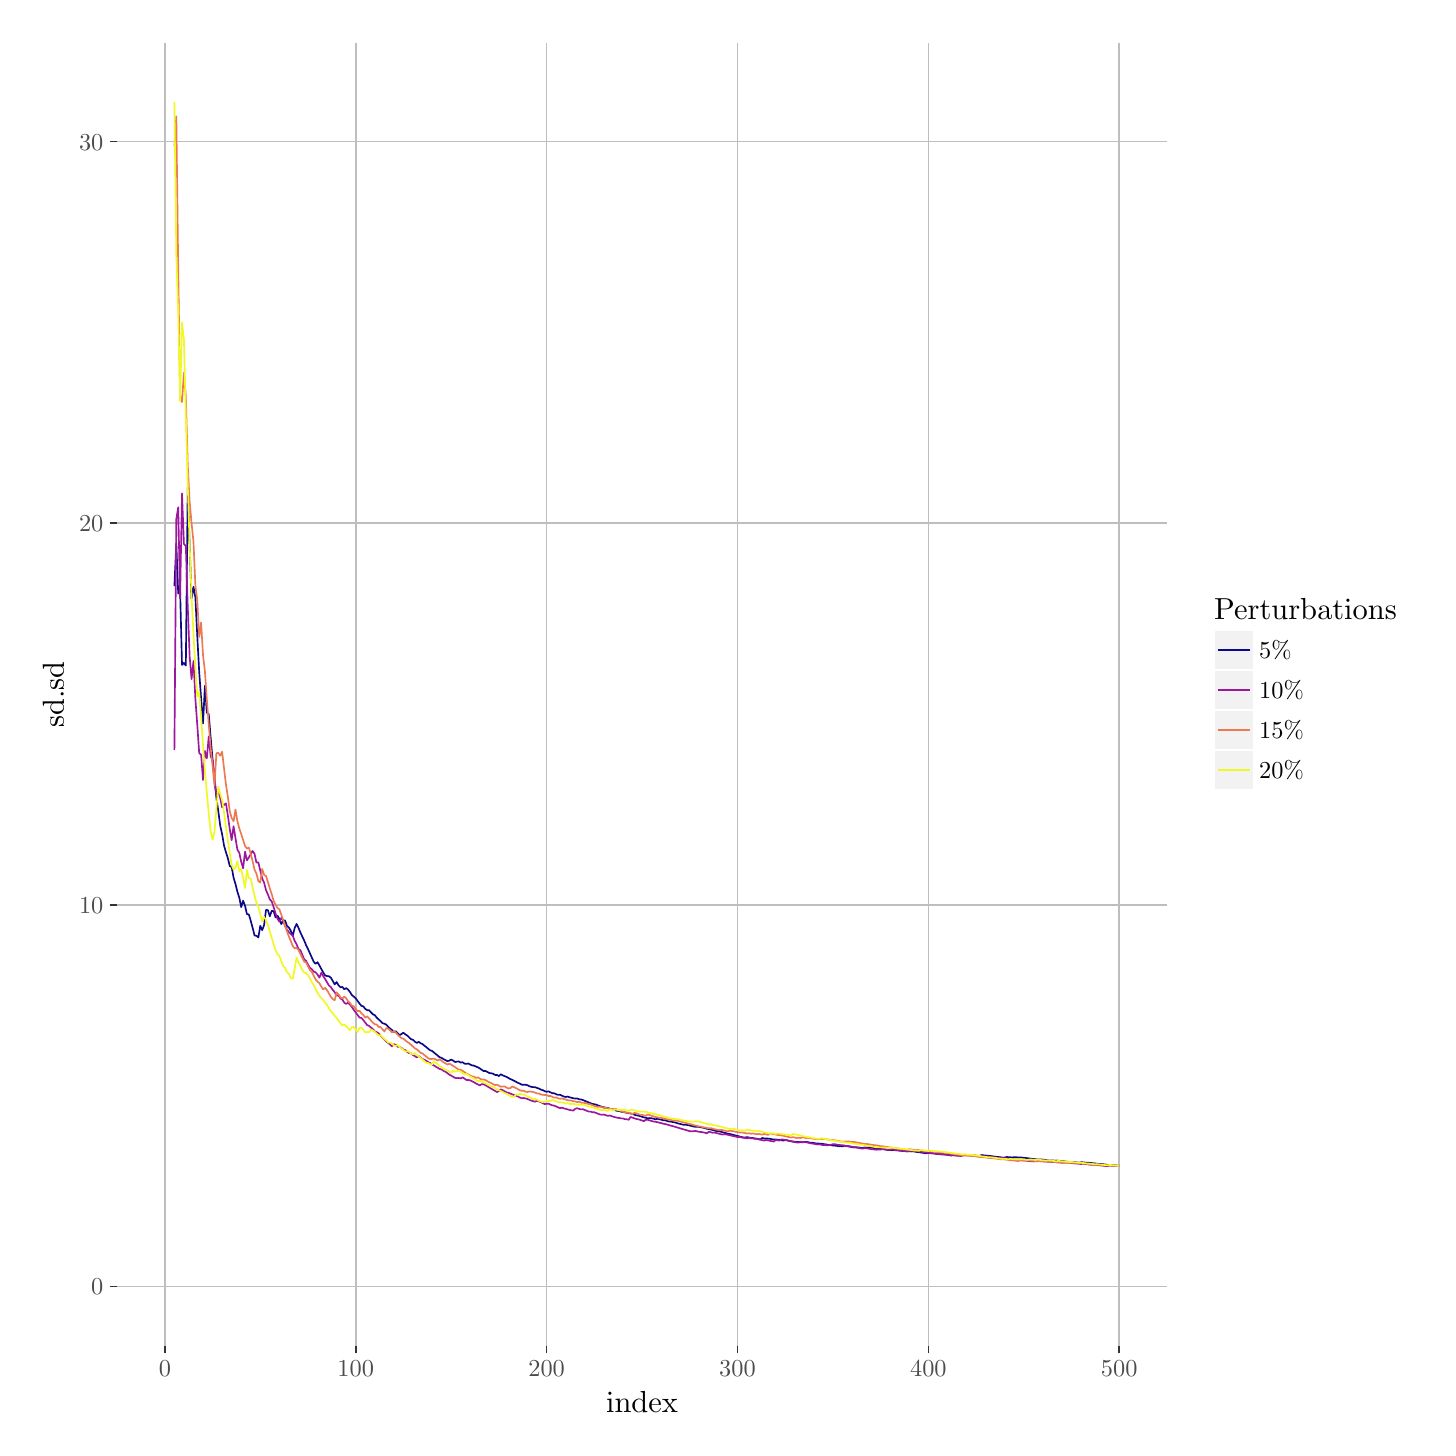
\begin{tikzpicture}[x=1pt,y=1pt]
\definecolor{fillColor}{RGB}{255,255,255}
\path[use as bounding box,fill=fillColor,fill opacity=0.00] (0,0) rectangle (505.89,505.89);
\begin{scope}
\path[clip] (  0.00,  0.00) rectangle (505.89,505.89);
\definecolor{drawColor}{RGB}{255,255,255}
\definecolor{fillColor}{RGB}{255,255,255}

\path[draw=drawColor,line width= 0.6pt,line join=round,line cap=round,fill=fillColor] (  0.00,  0.00) rectangle (505.89,505.89);
\end{scope}
\begin{scope}
\path[clip] ( 32.32, 29.59) rectangle (411.67,500.39);
\definecolor{drawColor}{RGB}{190,190,190}

\path[draw=drawColor,line width= 0.6pt,line join=round] ( 32.32, 50.99) --
	(411.67, 50.99);

\path[draw=drawColor,line width= 0.6pt,line join=round] ( 32.32,188.89) --
	(411.67,188.89);

\path[draw=drawColor,line width= 0.6pt,line join=round] ( 32.32,326.80) --
	(411.67,326.80);

\path[draw=drawColor,line width= 0.6pt,line join=round] ( 32.32,464.71) --
	(411.67,464.71);

\path[draw=drawColor,line width= 0.6pt,line join=round] ( 49.57, 29.59) --
	( 49.57,500.39);

\path[draw=drawColor,line width= 0.6pt,line join=round] (118.54, 29.59) --
	(118.54,500.39);

\path[draw=drawColor,line width= 0.6pt,line join=round] (187.51, 29.59) --
	(187.51,500.39);

\path[draw=drawColor,line width= 0.6pt,line join=round] (256.49, 29.59) --
	(256.49,500.39);

\path[draw=drawColor,line width= 0.6pt,line join=round] (325.46, 29.59) --
	(325.46,500.39);

\path[draw=drawColor,line width= 0.6pt,line join=round] (394.43, 29.59) --
	(394.43,500.39);
\definecolor{drawColor}{RGB}{13,8,135}

\path[draw=drawColor,line width= 0.6pt,line join=round] ( 53.02,304.12) --
	( 53.71,319.53) --
	( 54.40,301.41) --
	( 55.08,302.66) --
	( 55.77,275.61) --
	( 56.46,276.35) --
	( 57.15,275.39) --
	( 57.84,339.70) --
	( 58.53,318.60) --
	( 59.22,299.51) --
	( 59.91,303.85) --
	( 60.60,300.01) --
	( 61.29,285.98) --
	( 61.98,273.08) --
	( 62.67,263.59) --
	( 63.36,254.46) --
	( 64.05,268.08) --
	( 64.74,258.38) --
	( 65.43,257.81) --
	( 66.12,249.37) --
	( 66.81,241.55) --
	( 67.50,234.23) --
	( 68.19,227.53) --
	( 68.88,222.85) --
	( 69.57,217.54) --
	( 70.26,214.48) --
	( 70.95,210.35) --
	( 71.64,207.96) --
	( 72.33,205.77) --
	( 73.02,202.97) --
	( 73.71,202.56) --
	( 74.40,198.75) --
	( 75.09,196.45) --
	( 75.78,193.66) --
	( 76.47,191.53) --
	( 77.16,188.10) --
	( 77.85,190.41) --
	( 78.54,188.59) --
	( 79.23,185.57) --
	( 79.92,185.47) --
	( 80.60,183.20) --
	( 81.29,180.59) --
	( 81.98,177.86) --
	( 82.67,177.74) --
	( 83.36,177.13) --
	( 84.05,181.33) --
	( 84.74,179.78) --
	( 85.43,181.63) --
	( 86.12,187.08) --
	( 86.81,187.01) --
	( 87.50,184.78) --
	( 88.19,186.78) --
	( 88.88,186.62) --
	( 89.57,184.40) --
	( 90.26,184.99) --
	( 90.95,183.86) --
	( 91.64,181.97) --
	( 92.33,183.28) --
	( 93.02,183.27) --
	( 93.71,181.28) --
	( 94.40,180.70) --
	( 95.09,179.55) --
	( 95.78,177.67) --
	( 96.47,180.53) --
	( 97.16,182.02) --
	( 97.85,180.63) --
	( 98.54,178.93) --
	( 99.23,177.48) --
	( 99.92,176.03) --
	(100.61,174.35) --
	(101.30,172.92) --
	(101.99,171.43) --
	(102.68,169.87) --
	(103.37,168.35) --
	(104.06,167.60) --
	(104.75,168.20) --
	(105.43,166.99) --
	(106.12,165.71) --
	(106.81,164.47) --
	(107.50,163.39) --
	(108.19,163.19) --
	(108.88,163.12) --
	(109.57,162.57) --
	(110.26,161.38) --
	(110.95,160.19) --
	(111.64,161.03) --
	(112.33,159.87) --
	(113.02,159.14) --
	(113.71,159.25) --
	(114.40,158.42) --
	(115.09,158.83) --
	(115.78,158.30) --
	(116.47,157.40) --
	(117.16,156.32) --
	(117.85,155.75) --
	(118.54,155.14) --
	(119.23,154.18) --
	(119.92,153.23) --
	(120.61,152.42) --
	(121.30,152.22) --
	(121.99,151.32) --
	(122.68,150.85) --
	(123.37,150.85) --
	(124.06,150.07) --
	(124.75,149.36) --
	(125.44,149.05) --
	(126.13,148.16) --
	(126.82,147.51) --
	(127.51,146.92) --
	(128.20,146.16) --
	(128.89,145.97) --
	(129.58,145.64) --
	(130.27,144.84) --
	(130.95,144.23) --
	(131.64,143.71) --
	(132.33,142.98) --
	(133.02,143.20) --
	(133.71,142.56) --
	(134.40,141.83) --
	(135.09,142.28) --
	(135.78,142.71) --
	(136.47,142.12) --
	(137.16,141.70) --
	(137.85,141.00) --
	(138.54,140.37) --
	(139.23,140.15) --
	(139.92,139.47) --
	(140.61,139.04) --
	(141.30,139.43) --
	(141.99,138.90) --
	(142.68,138.63) --
	(143.37,137.99) --
	(144.06,137.51) --
	(144.75,136.89) --
	(145.44,136.36) --
	(146.13,136.14) --
	(146.82,135.54) --
	(147.51,134.99) --
	(148.20,134.41) --
	(148.89,133.83) --
	(149.58,133.63) --
	(150.27,133.15) --
	(150.96,132.81) --
	(151.65,132.48) --
	(152.34,132.60) --
	(153.03,133.03) --
	(153.72,132.67) --
	(154.41,132.13) --
	(155.10,132.27) --
	(155.79,132.31) --
	(156.47,131.92) --
	(157.16,132.06) --
	(157.85,131.54) --
	(158.54,131.45) --
	(159.23,131.60) --
	(159.92,131.19) --
	(160.61,130.90) --
	(161.30,130.83) --
	(161.99,130.48) --
	(162.68,130.21) --
	(163.37,129.81) --
	(164.06,129.33) --
	(164.75,128.86) --
	(165.44,128.91) --
	(166.13,128.52) --
	(166.82,128.15) --
	(167.51,128.07) --
	(168.20,127.87) --
	(168.89,127.46) --
	(169.58,127.46) --
	(170.27,127.03) --
	(170.96,127.69) --
	(171.65,127.32) --
	(172.34,127.02) --
	(173.03,126.76) --
	(173.72,126.36) --
	(174.41,125.96) --
	(175.10,125.69) --
	(175.79,125.32) --
	(176.48,124.98) --
	(177.17,124.59) --
	(177.86,124.31) --
	(178.55,123.93) --
	(179.24,123.93) --
	(179.93,123.94) --
	(180.62,123.74) --
	(181.31,123.37) --
	(181.99,123.15) --
	(182.68,123.06) --
	(183.37,123.02) --
	(184.06,122.76) --
	(184.75,122.52) --
	(185.44,122.16) --
	(186.13,121.95) --
	(186.82,121.60) --
	(187.51,121.38) --
	(188.20,121.54) --
	(188.89,121.19) --
	(189.58,120.86) --
	(190.27,120.82) --
	(190.96,120.49) --
	(191.65,120.25) --
	(192.34,120.29) --
	(193.03,119.98) --
	(193.72,119.66) --
	(194.41,119.49) --
	(195.10,119.65) --
	(195.79,119.39) --
	(196.48,119.23) --
	(197.17,119.02) --
	(197.86,118.94) --
	(198.55,118.97) --
	(199.24,118.66) --
	(199.93,118.60) --
	(200.62,118.40) --
	(201.31,118.10) --
	(202.00,117.82) --
	(202.69,117.54) --
	(203.38,117.25) --
	(204.07,116.97) --
	(204.76,116.88) --
	(205.45,116.71) --
	(206.14,116.43) --
	(206.82,116.19) --
	(207.51,115.92) --
	(208.20,115.77) --
	(208.89,115.62) --
	(209.58,115.50) --
	(210.27,115.31) --
	(210.96,115.11) --
	(211.65,114.94) --
	(212.34,114.67) --
	(213.03,114.48) --
	(213.72,114.42) --
	(214.41,114.19) --
	(215.10,114.09) --
	(215.79,113.93) --
	(216.48,113.79) --
	(217.17,113.59) --
	(217.86,113.55) --
	(218.55,113.33) --
	(219.24,113.09) --
	(219.93,112.87) --
	(220.62,112.78) --
	(221.31,112.56) --
	(222.00,112.33) --
	(222.69,112.13) --
	(223.38,111.98) --
	(224.07,111.77) --
	(224.76,111.88) --
	(225.45,111.80) --
	(226.14,111.65) --
	(226.83,111.42) --
	(227.52,111.63) --
	(228.21,111.42) --
	(228.90,111.30) --
	(229.59,111.09) --
	(230.28,111.07) --
	(230.97,110.85) --
	(231.66,110.63) --
	(232.34,110.60) --
	(233.03,110.45) --
	(233.72,110.34) --
	(234.41,110.13) --
	(235.10,109.91) --
	(235.79,109.76) --
	(236.48,109.58) --
	(237.17,109.40) --
	(237.86,109.43) --
	(238.55,109.37) --
	(239.24,109.17) --
	(239.93,109.02) --
	(240.62,108.81) --
	(241.31,108.73) --
	(242.00,108.75) --
	(242.69,108.65) --
	(243.38,108.54) --
	(244.07,108.39) --
	(244.76,108.20) --
	(245.45,108.01) --
	(246.14,107.89) --
	(246.83,107.75) --
	(247.52,107.57) --
	(248.21,107.39) --
	(248.90,107.19) --
	(249.59,107.16) --
	(250.28,106.98) --
	(250.97,106.79) --
	(251.66,106.60) --
	(252.35,106.41) --
	(253.04,106.23) --
	(253.73,106.12) --
	(254.42,105.95) --
	(255.11,105.77) --
	(255.80,105.59) --
	(256.49,105.41) --
	(257.18,105.23) --
	(257.86,105.05) --
	(258.55,104.90) --
	(259.24,104.83) --
	(259.93,105.01) --
	(260.62,104.85) --
	(261.31,104.68) --
	(262.00,104.67) --
	(262.69,104.51) --
	(263.38,104.43) --
	(264.07,104.31) --
	(264.76,104.17) --
	(265.45,104.67) --
	(266.14,104.51) --
	(266.83,104.52) --
	(267.52,104.46) --
	(268.21,104.37) --
	(268.90,104.24) --
	(269.59,104.09) --
	(270.28,104.17) --
	(270.97,104.01) --
	(271.66,104.02) --
	(272.35,103.88) --
	(273.04,103.72) --
	(273.73,103.97) --
	(274.42,103.82) --
	(275.11,103.66) --
	(275.80,103.50) --
	(276.49,103.41) --
	(277.18,103.31) --
	(277.87,103.25) --
	(278.56,103.27) --
	(279.25,103.22) --
	(279.94,103.07) --
	(280.63,103.22) --
	(281.32,103.25) --
	(282.01,103.15) --
	(282.70,103.00) --
	(283.38,102.99) --
	(284.07,102.88) --
	(284.76,102.73) --
	(285.45,102.74) --
	(286.14,102.62) --
	(286.83,102.61) --
	(287.52,102.48) --
	(288.21,102.39) --
	(288.90,102.26) --
	(289.59,102.11) --
	(290.28,102.08) --
	(290.97,101.94) --
	(291.66,101.91) --
	(292.35,101.84) --
	(293.04,101.70) --
	(293.73,101.74) --
	(294.42,101.64) --
	(295.11,101.89) --
	(295.80,101.75) --
	(296.49,101.63) --
	(297.18,101.52) --
	(297.87,101.39) --
	(298.56,101.26) --
	(299.25,101.38) --
	(299.94,101.25) --
	(300.63,101.21) --
	(301.32,101.08) --
	(302.01,101.15) --
	(302.70,101.26) --
	(303.39,101.14) --
	(304.08,101.35) --
	(304.77,101.24) --
	(305.46,101.11) --
	(306.15,100.97) --
	(306.84,100.84) --
	(307.53,100.89) --
	(308.21,100.78) --
	(308.90,100.68) --
	(309.59,100.56) --
	(310.28,100.43) --
	(310.97,100.32) --
	(311.66,100.29) --
	(312.35,100.27) --
	(313.04,100.31) --
	(313.73,100.23) --
	(314.42,100.25) --
	(315.11,100.13) --
	(315.80,100.05) --
	(316.49, 99.92) --
	(317.18, 99.92) --
	(317.87, 99.87) --
	(318.56, 99.94) --
	(319.25, 99.82) --
	(319.94, 99.85) --
	(320.63, 99.74) --
	(321.32, 99.62) --
	(322.01, 99.56) --
	(322.70, 99.44) --
	(323.39, 99.34) --
	(324.08, 99.23) --
	(324.77, 99.15) --
	(325.46, 99.26) --
	(326.15, 99.15) --
	(326.84, 99.17) --
	(327.53, 99.07) --
	(328.22, 98.97) --
	(328.91, 98.86) --
	(329.60, 98.82) --
	(330.29, 98.77) --
	(330.98, 98.79) --
	(331.67, 98.74) --
	(332.36, 98.63) --
	(333.05, 98.51) --
	(333.73, 98.44) --
	(334.42, 98.50) --
	(335.11, 98.50) --
	(335.80, 98.46) --
	(336.49, 98.38) --
	(337.18, 98.35) --
	(337.87, 98.35) --
	(338.56, 98.42) --
	(339.25, 98.57) --
	(339.94, 98.50) --
	(340.63, 98.45) --
	(341.32, 98.34) --
	(342.01, 98.38) --
	(342.70, 98.31) --
	(343.39, 98.20) --
	(344.08, 98.28) --
	(344.77, 98.52) --
	(345.46, 98.41) --
	(346.15, 98.35) --
	(346.84, 98.25) --
	(347.53, 98.22) --
	(348.22, 98.13) --
	(348.91, 98.03) --
	(349.60, 97.93) --
	(350.29, 97.83) --
	(350.98, 97.78) --
	(351.67, 97.68) --
	(352.36, 97.58) --
	(353.05, 97.61) --
	(353.74, 97.80) --
	(354.43, 97.76) --
	(355.12, 97.69) --
	(355.81, 97.68) --
	(356.50, 97.71) --
	(357.19, 97.72) --
	(357.88, 97.65) --
	(358.57, 97.64) --
	(359.25, 97.60) --
	(359.94, 97.53) --
	(360.63, 97.45) --
	(361.32, 97.37) --
	(362.01, 97.27) --
	(362.70, 97.18) --
	(363.39, 97.08) --
	(364.08, 97.03) --
	(364.77, 96.93) --
	(365.46, 96.91) --
	(366.15, 96.92) --
	(366.84, 96.86) --
	(367.53, 96.78) --
	(368.22, 96.68) --
	(368.91, 96.61) --
	(369.60, 96.52) --
	(370.29, 96.58) --
	(370.98, 96.48) --
	(371.67, 96.53) --
	(372.36, 96.45) --
	(373.05, 96.41) --
	(373.74, 96.33) --
	(374.43, 96.25) --
	(375.12, 96.15) --
	(375.81, 96.07) --
	(376.50, 96.04) --
	(377.19, 95.94) --
	(377.88, 95.90) --
	(378.57, 95.91) --
	(379.26, 95.83) --
	(379.95, 95.74) --
	(380.64, 95.89) --
	(381.33, 95.88) --
	(382.02, 95.80) --
	(382.71, 95.71) --
	(383.40, 95.73) --
	(384.08, 95.65) --
	(384.77, 95.59) --
	(385.46, 95.51) --
	(386.15, 95.42) --
	(386.84, 95.33) --
	(387.53, 95.30) --
	(388.22, 95.22) --
	(388.91, 95.15) --
	(389.60, 95.06) --
	(390.29, 94.97) --
	(390.98, 94.89) --
	(391.67, 94.83) --
	(392.36, 94.83) --
	(393.05, 94.75) --
	(393.74, 94.68) --
	(394.43, 94.60);
\definecolor{drawColor}{RGB}{156,23,158}

\path[draw=drawColor,line width= 0.6pt,line join=round] ( 53.02,244.93) --
	( 53.71,328.34) --
	( 54.40,332.57) --
	( 55.08,299.66) --
	( 55.77,337.58) --
	( 56.46,319.32) --
	( 57.15,318.60) --
	( 57.84,296.79) --
	( 58.53,278.61) --
	( 59.22,270.49) --
	( 59.91,277.04) --
	( 60.60,263.39) --
	( 61.29,253.95) --
	( 61.98,243.73) --
	( 62.67,243.16) --
	( 63.36,234.03) --
	( 64.05,244.53) --
	( 64.74,241.85) --
	( 65.43,249.77) --
	( 66.12,242.59) --
	( 66.81,241.32) --
	( 67.50,235.19) --
	( 68.19,228.40) --
	( 68.88,229.90) --
	( 69.57,227.55) --
	( 70.26,224.15) --
	( 70.95,225.05) --
	( 71.64,225.57) --
	( 72.33,221.29) --
	( 73.02,216.28) --
	( 73.71,212.32) --
	( 74.40,217.33) --
	( 75.09,213.03) --
	( 75.78,208.82) --
	( 76.47,207.75) --
	( 77.16,204.46) --
	( 77.85,202.13) --
	( 78.54,208.13) --
	( 79.23,205.01) --
	( 79.92,206.06) --
	( 80.60,207.27) --
	( 81.29,208.39) --
	( 81.98,207.33) --
	( 82.67,204.17) --
	( 83.36,204.27) --
	( 84.05,201.30) --
	( 84.74,198.46) --
	( 85.43,196.94) --
	( 86.12,194.23) --
	( 86.81,192.65) --
	( 87.50,190.89) --
	( 88.19,190.15) --
	( 88.88,188.10) --
	( 89.57,185.84) --
	( 90.26,183.88) --
	( 90.95,182.83) --
	( 91.64,184.24) --
	( 92.33,183.23) --
	( 93.02,181.25) --
	( 93.71,179.95) --
	( 94.40,179.07) --
	( 95.09,178.36) --
	( 95.78,177.79) --
	( 96.47,175.93) --
	( 97.16,174.69) --
	( 97.85,172.97) --
	( 98.54,172.55) --
	( 99.23,170.89) --
	( 99.92,169.25) --
	(100.61,168.65) --
	(101.30,167.35) --
	(101.99,166.16) --
	(102.68,165.66) --
	(103.37,164.76) --
	(104.06,164.55) --
	(104.75,163.69) --
	(105.43,162.62) --
	(106.12,164.41) --
	(106.81,163.11) --
	(107.50,162.10) --
	(108.19,160.89) --
	(108.88,159.77) --
	(109.57,159.18) --
	(110.26,158.13) --
	(110.95,157.35) --
	(111.64,156.17) --
	(112.33,156.18) --
	(113.02,155.08) --
	(113.71,154.69) --
	(114.40,153.59) --
	(115.09,153.14) --
	(115.78,153.56) --
	(116.47,152.84) --
	(117.16,151.96) --
	(117.85,150.96) --
	(118.54,150.05) --
	(119.23,149.10) --
	(119.92,148.18) --
	(120.61,148.06) --
	(121.30,147.26) --
	(121.99,146.35) --
	(122.68,145.46) --
	(123.37,145.19) --
	(124.06,144.56) --
	(124.75,144.02) --
	(125.44,143.20) --
	(126.13,142.89) --
	(126.82,142.49) --
	(127.51,141.70) --
	(128.20,140.96) --
	(128.89,140.24) --
	(129.58,139.54) --
	(130.27,139.01) --
	(130.95,138.47) --
	(131.64,137.79) --
	(132.33,138.56) --
	(133.02,138.34) --
	(133.71,137.63) --
	(134.40,137.55) --
	(135.09,137.22) --
	(135.78,136.63) --
	(136.47,136.40) --
	(137.16,135.74) --
	(137.85,135.36) --
	(138.54,135.23) --
	(139.23,134.61) --
	(139.92,134.25) --
	(140.61,133.78) --
	(141.30,134.25) --
	(141.99,133.73) --
	(142.68,133.21) --
	(143.37,132.91) --
	(144.06,132.58) --
	(144.75,132.07) --
	(145.44,131.78) --
	(146.13,131.21) --
	(146.82,130.89) --
	(147.51,130.41) --
	(148.20,130.02) --
	(148.89,129.59) --
	(149.58,129.44) --
	(150.27,128.93) --
	(150.96,128.61) --
	(151.65,128.10) --
	(152.34,127.58) --
	(153.03,127.23) --
	(153.72,126.80) --
	(154.41,126.41) --
	(155.10,126.31) --
	(155.79,126.35) --
	(156.47,126.19) --
	(157.16,126.57) --
	(157.85,126.12) --
	(158.54,125.65) --
	(159.23,125.61) --
	(159.92,125.52) --
	(160.61,125.15) --
	(161.30,124.81) --
	(161.99,124.36) --
	(162.68,124.05) --
	(163.37,123.63) --
	(164.06,124.16) --
	(164.75,124.04) --
	(165.44,123.74) --
	(166.13,123.31) --
	(166.82,122.90) --
	(167.51,122.48) --
	(168.20,122.09) --
	(168.89,121.68) --
	(169.58,121.27) --
	(170.27,121.60) --
	(170.96,122.23) --
	(171.65,121.94) --
	(172.34,121.55) --
	(173.03,121.16) --
	(173.72,121.03) --
	(174.41,120.73) --
	(175.10,120.43) --
	(175.79,120.22) --
	(176.48,119.93) --
	(177.17,119.66) --
	(177.86,119.29) --
	(178.55,119.05) --
	(179.24,119.12) --
	(179.93,118.96) --
	(180.62,118.77) --
	(181.31,118.45) --
	(181.99,118.17) --
	(182.68,117.96) --
	(183.37,117.79) --
	(184.06,118.13) --
	(184.75,117.93) --
	(185.44,117.59) --
	(186.13,117.27) --
	(186.82,116.94) --
	(187.51,117.02) --
	(188.20,117.06) --
	(188.89,116.74) --
	(189.58,116.46) --
	(190.27,116.38) --
	(190.96,116.07) --
	(191.65,115.76) --
	(192.34,115.47) --
	(193.03,115.66) --
	(193.72,115.37) --
	(194.41,115.20) --
	(195.10,115.02) --
	(195.79,114.82) --
	(196.48,114.68) --
	(197.17,114.60) --
	(197.86,115.23) --
	(198.55,115.43) --
	(199.24,115.20) --
	(199.93,115.00) --
	(200.62,115.07) --
	(201.31,114.79) --
	(202.00,114.51) --
	(202.69,114.23) --
	(203.38,114.20) --
	(204.07,113.98) --
	(204.76,113.96) --
	(205.45,113.70) --
	(206.14,113.43) --
	(206.82,113.16) --
	(207.51,113.08) --
	(208.20,113.15) --
	(208.89,112.91) --
	(209.58,112.67) --
	(210.27,112.80) --
	(210.96,112.59) --
	(211.65,112.34) --
	(212.34,112.16) --
	(213.03,111.99) --
	(213.72,111.91) --
	(214.41,111.77) --
	(215.10,111.74) --
	(215.79,111.50) --
	(216.48,111.45) --
	(217.17,111.25) --
	(217.86,112.27) --
	(218.55,112.03) --
	(219.24,111.80) --
	(219.93,111.56) --
	(220.62,111.44) --
	(221.31,111.22) --
	(222.00,110.98) --
	(222.69,110.74) --
	(223.38,111.30) --
	(224.07,111.22) --
	(224.76,111.03) --
	(225.45,110.80) --
	(226.14,110.63) --
	(226.83,110.54) --
	(227.52,110.40) --
	(228.21,110.21) --
	(228.90,110.07) --
	(229.59,109.85) --
	(230.28,109.72) --
	(230.97,109.55) --
	(231.66,109.36) --
	(232.34,109.14) --
	(233.03,108.98) --
	(233.72,108.78) --
	(234.41,108.57) --
	(235.10,108.36) --
	(235.79,108.15) --
	(236.48,107.94) --
	(237.17,107.75) --
	(237.86,107.55) --
	(238.55,107.34) --
	(239.24,107.14) --
	(239.93,107.07) --
	(240.62,107.12) --
	(241.31,107.23) --
	(242.00,107.03) --
	(242.69,106.89) --
	(243.38,106.84) --
	(244.07,106.73) --
	(244.76,106.56) --
	(245.45,106.37) --
	(246.14,106.94) --
	(246.83,106.76) --
	(247.52,106.57) --
	(248.21,106.65) --
	(248.90,106.46) --
	(249.59,106.28) --
	(250.28,106.09) --
	(250.97,105.91) --
	(251.66,106.05) --
	(252.35,105.95) --
	(253.04,105.82) --
	(253.73,105.67) --
	(254.42,105.48) --
	(255.11,105.32) --
	(255.80,105.18) --
	(256.49,105.00) --
	(257.18,105.06) --
	(257.86,104.90) --
	(258.55,104.75) --
	(259.24,104.67) --
	(259.93,104.53) --
	(260.62,104.70) --
	(261.31,104.57) --
	(262.00,104.53) --
	(262.69,104.42) --
	(263.38,104.37) --
	(264.07,104.20) --
	(264.76,104.04) --
	(265.45,103.89) --
	(266.14,103.74) --
	(266.83,103.96) --
	(267.52,103.82) --
	(268.21,103.66) --
	(268.90,103.53) --
	(269.59,103.39) --
	(270.28,103.93) --
	(270.97,103.87) --
	(271.66,103.74) --
	(272.35,104.15) --
	(273.04,104.10) --
	(273.73,103.94) --
	(274.42,103.82) --
	(275.11,103.66) --
	(275.80,103.51) --
	(276.49,103.35) --
	(277.18,103.20) --
	(277.87,103.08) --
	(278.56,102.99) --
	(279.25,103.30) --
	(279.94,103.23) --
	(280.63,103.22) --
	(281.32,103.12) --
	(282.01,102.97) --
	(282.70,102.82) --
	(283.38,102.67) --
	(284.07,102.60) --
	(284.76,102.45) --
	(285.45,102.34) --
	(286.14,102.38) --
	(286.83,102.23) --
	(287.52,102.09) --
	(288.21,102.14) --
	(288.90,101.99) --
	(289.59,102.12) --
	(290.28,102.22) --
	(290.97,102.43) --
	(291.66,102.43) --
	(292.35,102.30) --
	(293.04,102.17) --
	(293.73,102.11) --
	(294.42,102.06) --
	(295.11,101.93) --
	(295.80,101.79) --
	(296.49,101.79) --
	(297.18,101.65) --
	(297.87,101.51) --
	(298.56,101.40) --
	(299.25,101.26) --
	(299.94,101.13) --
	(300.63,101.00) --
	(301.32,100.87) --
	(302.01,100.88) --
	(302.70,101.02) --
	(303.39,100.89) --
	(304.08,100.78) --
	(304.77,100.65) --
	(305.46,100.56) --
	(306.15,100.53) --
	(306.84,100.43) --
	(307.53,100.55) --
	(308.21,100.48) --
	(308.90,100.71) --
	(309.59,100.58) --
	(310.28,100.52) --
	(310.97,100.43) --
	(311.66,100.43) --
	(312.35,100.54) --
	(313.04,100.41) --
	(313.73,100.28) --
	(314.42,100.21) --
	(315.11,100.08) --
	(315.80,100.11) --
	(316.49, 99.99) --
	(317.18, 99.90) --
	(317.87, 99.84) --
	(318.56, 99.85) --
	(319.25,100.13) --
	(319.94,100.01) --
	(320.63, 99.90) --
	(321.32, 99.88) --
	(322.01, 99.81) --
	(322.70, 99.74) --
	(323.39, 99.62) --
	(324.08, 99.50) --
	(324.77, 99.39) --
	(325.46, 99.32) --
	(326.15, 99.20) --
	(326.84, 99.17) --
	(327.53, 99.11) --
	(328.22, 99.02) --
	(328.91, 98.97) --
	(329.60, 98.85) --
	(330.29, 98.75) --
	(330.98, 98.70) --
	(331.67, 98.61) --
	(332.36, 98.52) --
	(333.05, 98.43) --
	(333.73, 98.34) --
	(334.42, 98.43) --
	(335.11, 98.31) --
	(335.80, 98.27) --
	(336.49, 98.24) --
	(337.18, 98.13) --
	(337.87, 98.50) --
	(338.56, 98.50) --
	(339.25, 98.39) --
	(339.94, 98.46) --
	(340.63, 98.35) --
	(341.32, 98.28) --
	(342.01, 98.24) --
	(342.70, 98.14) --
	(343.39, 98.07) --
	(344.08, 97.98) --
	(344.77, 97.97) --
	(345.46, 98.11) --
	(346.15, 98.01) --
	(346.84, 98.03) --
	(347.53, 97.92) --
	(348.22, 97.82) --
	(348.91, 97.74) --
	(349.60, 97.63) --
	(350.29, 97.53) --
	(350.98, 97.48) --
	(351.67, 97.45) --
	(352.36, 97.46) --
	(353.05, 97.36) --
	(353.74, 97.29) --
	(354.43, 97.21) --
	(355.12, 97.11) --
	(355.81, 97.03) --
	(356.50, 96.95) --
	(357.19, 96.87) --
	(357.88, 96.79) --
	(358.57, 96.71) --
	(359.25, 96.63) --
	(359.94, 96.55) --
	(360.63, 96.49) --
	(361.32, 96.40) --
	(362.01, 96.31) --
	(362.70, 96.26) --
	(363.39, 96.20) --
	(364.08, 96.28) --
	(364.77, 96.21) --
	(365.46, 96.35) --
	(366.15, 96.26) --
	(366.84, 96.22) --
	(367.53, 96.16) --
	(368.22, 96.12) --
	(368.91, 96.09) --
	(369.60, 96.06) --
	(370.29, 95.97) --
	(370.98, 96.02) --
	(371.67, 95.93) --
	(372.36, 95.85) --
	(373.05, 95.86) --
	(373.74, 95.84) --
	(374.43, 95.75) --
	(375.12, 95.84) --
	(375.81, 95.81) --
	(376.50, 95.72) --
	(377.19, 95.63) --
	(377.88, 95.53) --
	(378.57, 95.47) --
	(379.26, 95.44) --
	(379.95, 95.35) --
	(380.64, 95.27) --
	(381.33, 95.36) --
	(382.02, 95.27) --
	(382.71, 95.18) --
	(383.40, 95.10) --
	(384.08, 95.03) --
	(384.77, 95.01) --
	(385.46, 95.00) --
	(386.15, 94.95) --
	(386.84, 94.87) --
	(387.53, 94.78) --
	(388.22, 94.70) --
	(388.91, 94.63) --
	(389.60, 94.54) --
	(390.29, 94.55) --
	(390.98, 94.69) --
	(391.67, 94.67) --
	(392.36, 94.60) --
	(393.05, 94.72) --
	(393.74, 94.66) --
	(394.43, 94.60);
\definecolor{drawColor}{RGB}{237,121,83}

\path[draw=drawColor,line width= 0.6pt,line join=round] ( 53.02,463.12) --
	( 53.71,473.85) --
	( 54.40,418.90) --
	( 55.08,373.02) --
	( 55.77,370.62) --
	( 56.46,381.22) --
	( 57.15,372.68) --
	( 57.84,347.95) --
	( 58.53,334.56) --
	( 59.22,326.83) --
	( 59.91,320.23) --
	( 60.60,304.31) --
	( 61.29,298.87) --
	( 61.98,285.65) --
	( 62.67,290.95) --
	( 63.36,279.13) --
	( 64.05,273.23) --
	( 64.74,263.14) --
	( 65.43,254.09) --
	( 66.12,245.66) --
	( 66.81,239.21) --
	( 67.50,232.01) --
	( 68.19,243.74) --
	( 68.88,243.82) --
	( 69.57,242.80) --
	( 70.26,244.24) --
	( 70.95,238.29) --
	( 71.64,232.44) --
	( 72.33,228.02) --
	( 73.02,222.82) --
	( 73.71,220.28) --
	( 74.40,219.14) --
	( 75.09,223.39) --
	( 75.78,219.14) --
	( 76.47,216.53) --
	( 77.16,214.53) --
	( 77.85,212.37) --
	( 78.54,210.24) --
	( 79.23,209.23) --
	( 79.92,209.64) --
	( 80.60,207.37) --
	( 81.29,204.67) --
	( 81.98,201.62) --
	( 82.67,200.18) --
	( 83.36,197.49) --
	( 84.05,196.99) --
	( 84.74,201.89) --
	( 85.43,199.72) --
	( 86.12,199.35) --
	( 86.81,197.19) --
	( 87.50,194.79) --
	( 88.19,192.80) --
	( 88.88,190.34) --
	( 89.57,189.03) --
	( 90.26,187.76) --
	( 90.95,187.33) --
	( 91.64,185.37) --
	( 92.33,183.41) --
	( 93.02,181.31) --
	( 93.71,179.30) --
	( 94.40,177.41) --
	( 95.09,175.83) --
	( 95.78,174.01) --
	( 96.47,173.24) --
	( 97.16,173.36) --
	( 97.85,172.66) --
	( 98.54,171.24) --
	( 99.23,169.78) --
	( 99.92,168.41) --
	(100.61,168.13) --
	(101.30,166.74) --
	(101.99,165.33) --
	(102.68,164.72) --
	(103.37,163.33) --
	(104.06,161.96) --
	(104.75,161.17) --
	(105.43,160.61) --
	(106.12,159.32) --
	(106.81,158.36) --
	(107.50,158.93) --
	(108.19,158.07) --
	(108.88,156.84) --
	(109.57,155.69) --
	(110.26,154.87) --
	(110.95,154.46) --
	(111.64,157.32) --
	(112.33,156.61) --
	(113.02,155.47) --
	(113.71,155.07) --
	(114.40,155.75) --
	(115.09,155.16) --
	(115.78,154.07) --
	(116.47,153.50) --
	(117.16,152.45) --
	(117.85,152.25) --
	(118.54,151.26) --
	(119.23,150.52) --
	(119.92,150.62) --
	(120.61,149.74) --
	(121.30,149.08) --
	(121.99,148.15) --
	(122.68,148.62) --
	(123.37,147.88) --
	(124.06,147.09) --
	(124.75,146.32) --
	(125.44,145.77) --
	(126.13,145.66) --
	(126.82,144.81) --
	(127.51,144.77) --
	(128.20,143.96) --
	(128.89,143.16) --
	(129.58,144.34) --
	(130.27,144.19) --
	(130.95,143.58) --
	(131.64,142.80) --
	(132.33,143.35) --
	(133.02,142.75) --
	(133.71,142.01) --
	(134.40,141.36) --
	(135.09,140.72) --
	(135.78,140.57) --
	(136.47,139.94) --
	(137.16,139.39) --
	(137.85,138.95) --
	(138.54,138.37) --
	(139.23,137.71) --
	(139.92,137.05) --
	(140.61,136.73) --
	(141.30,136.09) --
	(141.99,135.46) --
	(142.68,135.24) --
	(143.37,134.63) --
	(144.06,134.05) --
	(144.75,133.51) --
	(145.44,133.17) --
	(146.13,133.25) --
	(146.82,133.38) --
	(147.51,133.00) --
	(148.20,132.65) --
	(148.89,133.10) --
	(149.58,132.57) --
	(150.27,132.04) --
	(150.96,131.69) --
	(151.65,131.20) --
	(152.34,131.50) --
	(153.03,131.23) --
	(153.72,130.72) --
	(154.41,130.30) --
	(155.10,129.83) --
	(155.79,129.34) --
	(156.47,129.30) --
	(157.16,128.95) --
	(157.85,128.46) --
	(158.54,127.97) --
	(159.23,127.61) --
	(159.92,127.24) --
	(160.61,126.93) --
	(161.30,126.84) --
	(161.99,126.41) --
	(162.68,126.56) --
	(163.37,126.15) --
	(164.06,125.76) --
	(164.75,125.87) --
	(165.44,125.58) --
	(166.13,125.18) --
	(166.82,124.79) --
	(167.51,124.53) --
	(168.20,124.10) --
	(168.89,123.77) --
	(169.58,123.92) --
	(170.27,123.59) --
	(170.96,123.19) --
	(171.65,123.29) --
	(172.34,123.30) --
	(173.03,122.91) --
	(173.72,122.58) --
	(174.41,122.68) --
	(175.10,123.31) --
	(175.79,123.04) --
	(176.48,122.68) --
	(177.17,122.31) --
	(177.86,121.95) --
	(178.55,121.71) --
	(179.24,121.76) --
	(179.93,121.39) --
	(180.62,121.31) --
	(181.31,121.48) --
	(181.99,121.41) --
	(182.68,121.31) --
	(183.37,121.07) --
	(184.06,120.76) --
	(184.75,120.76) --
	(185.44,120.41) --
	(186.13,120.28) --
	(186.82,120.21) --
	(187.51,120.17) --
	(188.20,119.85) --
	(188.89,119.85) --
	(189.58,119.56) --
	(190.27,119.24) --
	(190.96,119.35) --
	(191.65,119.02) --
	(192.34,118.83) --
	(193.03,119.01) --
	(193.72,118.71) --
	(194.41,118.61) --
	(195.10,118.31) --
	(195.79,118.26) --
	(196.48,118.20) --
	(197.17,117.96) --
	(197.86,117.89) --
	(198.55,117.62) --
	(199.24,117.77) --
	(199.93,117.52) --
	(200.62,117.25) --
	(201.31,117.36) --
	(202.00,117.11) --
	(202.69,116.98) --
	(203.38,116.82) --
	(204.07,116.53) --
	(204.76,116.25) --
	(205.45,116.00) --
	(206.14,115.95) --
	(206.82,115.91) --
	(207.51,115.81) --
	(208.20,115.53) --
	(208.89,115.58) --
	(209.58,115.40) --
	(210.27,115.12) --
	(210.96,115.17) --
	(211.65,115.07) --
	(212.34,115.20) --
	(213.03,114.95) --
	(213.72,114.69) --
	(214.41,114.42) --
	(215.10,114.21) --
	(215.79,113.97) --
	(216.48,113.81) --
	(217.17,113.77) --
	(217.86,113.51) --
	(218.55,113.33) --
	(219.24,113.77) --
	(219.93,113.58) --
	(220.62,113.33) --
	(221.31,113.08) --
	(222.00,113.04) --
	(222.69,112.82) --
	(223.38,112.67) --
	(224.07,113.17) --
	(224.76,112.94) --
	(225.45,112.70) --
	(226.14,112.50) --
	(226.83,112.26) --
	(227.52,112.18) --
	(228.21,111.94) --
	(228.90,111.95) --
	(229.59,111.79) --
	(230.28,111.68) --
	(230.97,111.50) --
	(231.66,111.27) --
	(232.34,111.23) --
	(233.03,111.03) --
	(233.72,110.98) --
	(234.41,110.89) --
	(235.10,110.85) --
	(235.79,110.63) --
	(236.48,110.49) --
	(237.17,110.28) --
	(237.86,110.10) --
	(238.55,109.88) --
	(239.24,109.76) --
	(239.93,109.57) --
	(240.62,109.37) --
	(241.31,109.18) --
	(242.00,109.02) --
	(242.69,108.84) --
	(243.38,108.76) --
	(244.07,108.55) --
	(244.76,108.45) --
	(245.45,108.31) --
	(246.14,108.14) --
	(246.83,108.22) --
	(247.52,108.06) --
	(248.21,107.88) --
	(248.90,107.68) --
	(249.59,107.59) --
	(250.28,107.53) --
	(250.97,107.57) --
	(251.66,107.38) --
	(252.35,107.22) --
	(253.04,107.07) --
	(253.73,107.31) --
	(254.42,107.20) --
	(255.11,107.10) --
	(255.80,106.92) --
	(256.49,106.80) --
	(257.18,106.63) --
	(257.86,106.68) --
	(258.55,106.58) --
	(259.24,106.46) --
	(259.93,106.29) --
	(260.62,106.39) --
	(261.31,106.21) --
	(262.00,106.33) --
	(262.69,106.19) --
	(263.38,106.01) --
	(264.07,106.16) --
	(264.76,106.03) --
	(265.45,105.87) --
	(266.14,106.16) --
	(266.83,105.99) --
	(267.52,105.81) --
	(268.21,106.27) --
	(268.90,106.22) --
	(269.59,106.09) --
	(270.28,105.92) --
	(270.97,105.79) --
	(271.66,105.74) --
	(272.35,105.58) --
	(273.04,105.48) --
	(273.73,105.32) --
	(274.42,105.16) --
	(275.11,105.00) --
	(275.80,104.84) --
	(276.49,104.97) --
	(277.18,104.84) --
	(277.87,104.68) --
	(278.56,104.77) --
	(279.25,104.65) --
	(279.94,104.96) --
	(280.63,104.80) --
	(281.32,104.65) --
	(282.01,104.72) --
	(282.70,104.58) --
	(283.38,104.51) --
	(284.07,104.36) --
	(284.76,104.30) --
	(285.45,104.15) --
	(286.14,104.45) --
	(286.83,104.30) --
	(287.52,104.26) --
	(288.21,104.28) --
	(288.90,104.19) --
	(289.59,104.05) --
	(290.28,103.96) --
	(290.97,103.92) --
	(291.66,103.85) --
	(292.35,103.71) --
	(293.04,103.56) --
	(293.73,103.45) --
	(294.42,103.32) --
	(295.11,103.40) --
	(295.80,103.41) --
	(296.49,103.45) --
	(297.18,103.33) --
	(297.87,103.19) --
	(298.56,103.26) --
	(299.25,103.12) --
	(299.94,103.00) --
	(300.63,102.87) --
	(301.32,102.73) --
	(302.01,102.59) --
	(302.70,102.46) --
	(303.39,102.51) --
	(304.08,102.38) --
	(304.77,102.28) --
	(305.46,102.17) --
	(306.15,102.05) --
	(306.84,102.01) --
	(307.53,101.87) --
	(308.21,101.73) --
	(308.90,101.67) --
	(309.59,101.58) --
	(310.28,101.45) --
	(310.97,101.36) --
	(311.66,101.23) --
	(312.35,101.19) --
	(313.04,101.06) --
	(313.73,101.00) --
	(314.42,100.87) --
	(315.11,100.76) --
	(315.80,100.66) --
	(316.49,100.63) --
	(317.18,100.51) --
	(317.87,100.43) --
	(318.56,100.64) --
	(319.25,100.52) --
	(319.94,100.43) --
	(320.63,100.33) --
	(321.32,100.32) --
	(322.01,100.31) --
	(322.70,100.18) --
	(323.39,100.12) --
	(324.08,100.03) --
	(324.77, 99.96) --
	(325.46,100.04) --
	(326.15, 99.94) --
	(326.84, 99.82) --
	(327.53, 99.71) --
	(328.22, 99.61) --
	(328.91, 99.49) --
	(329.60, 99.55) --
	(330.29, 99.57) --
	(330.98, 99.45) --
	(331.67, 99.33) --
	(332.36, 99.24) --
	(333.05, 99.14) --
	(333.73, 99.04) --
	(334.42, 98.93) --
	(335.11, 98.81) --
	(335.80, 98.70) --
	(336.49, 98.61) --
	(337.18, 98.50) --
	(337.87, 98.41) --
	(338.56, 98.45) --
	(339.25, 98.34) --
	(339.94, 98.24) --
	(340.63, 98.32) --
	(341.32, 98.22) --
	(342.01, 98.11) --
	(342.70, 98.02) --
	(343.39, 97.91) --
	(344.08, 97.82) --
	(344.77, 97.75) --
	(345.46, 97.71) --
	(346.15, 97.64) --
	(346.84, 97.53) --
	(347.53, 97.43) --
	(348.22, 97.36) --
	(348.91, 97.36) --
	(349.60, 97.26) --
	(350.29, 97.17) --
	(350.98, 97.06) --
	(351.67, 96.97) --
	(352.36, 97.00) --
	(353.05, 96.93) --
	(353.74, 96.83) --
	(354.43, 96.73) --
	(355.12, 96.63) --
	(355.81, 96.62) --
	(356.50, 96.52) --
	(357.19, 96.43) --
	(357.88, 96.33) --
	(358.57, 96.52) --
	(359.25, 96.58) --
	(359.94, 96.48) --
	(360.63, 96.54) --
	(361.32, 96.60) --
	(362.01, 96.54) --
	(362.70, 96.46) --
	(363.39, 96.41) --
	(364.08, 96.38) --
	(364.77, 96.29) --
	(365.46, 96.34) --
	(366.15, 96.29) --
	(366.84, 96.34) --
	(367.53, 96.24) --
	(368.22, 96.25) --
	(368.91, 96.18) --
	(369.60, 96.19) --
	(370.29, 96.10) --
	(370.98, 96.01) --
	(371.67, 95.92) --
	(372.36, 95.84) --
	(373.05, 95.75) --
	(373.74, 95.66) --
	(374.43, 95.69) --
	(375.12, 95.69) --
	(375.81, 95.66) --
	(376.50, 95.77) --
	(377.19, 95.68) --
	(377.88, 95.67) --
	(378.57, 95.74) --
	(379.26, 95.66) --
	(379.95, 95.60) --
	(380.64, 95.54) --
	(381.33, 95.45) --
	(382.02, 95.36) --
	(382.71, 95.31) --
	(383.40, 95.24) --
	(384.08, 95.15) --
	(384.77, 95.07) --
	(385.46, 94.98) --
	(386.15, 94.95) --
	(386.84, 95.04) --
	(387.53, 94.98) --
	(388.22, 94.92) --
	(388.91, 94.84) --
	(389.60, 94.75) --
	(390.29, 94.79) --
	(390.98, 94.76) --
	(391.67, 94.74) --
	(392.36, 94.65) --
	(393.05, 94.59) --
	(393.74, 94.61) --
	(394.43, 94.60);
\definecolor{drawColor}{RGB}{240,249,33}

\path[draw=drawColor,line width= 0.6pt,line join=round] ( 53.02,478.99) --
	( 53.71,424.10) --
	( 54.40,402.62) --
	( 55.08,370.72) --
	( 55.77,399.35) --
	( 56.46,393.14) --
	( 57.15,365.76) --
	( 57.84,340.77) --
	( 58.53,318.74) --
	( 59.22,300.50) --
	( 59.91,286.77) --
	( 60.60,274.72) --
	( 61.29,264.15) --
	( 61.98,265.84) --
	( 62.67,256.80) --
	( 63.36,246.54) --
	( 64.05,237.33) --
	( 64.74,229.49) --
	( 65.43,221.86) --
	( 66.12,215.33) --
	( 66.81,212.47) --
	( 67.50,215.25) --
	( 68.19,223.69) --
	( 68.88,231.67) --
	( 69.57,229.04) --
	( 70.26,226.80) --
	( 70.95,222.44) --
	( 71.64,217.21) --
	( 72.33,212.18) --
	( 73.02,207.69) --
	( 73.71,203.35) --
	( 74.40,201.67) --
	( 75.09,202.21) --
	( 75.78,204.65) --
	( 76.47,201.11) --
	( 77.16,201.83) --
	( 77.85,198.52) --
	( 78.54,195.01) --
	( 79.23,201.54) --
	( 79.92,198.63) --
	( 80.60,198.35) --
	( 81.29,195.14) --
	( 81.98,192.21) --
	( 82.67,189.72) --
	( 83.36,188.20) --
	( 84.05,185.56) --
	( 84.74,182.98) --
	( 85.43,184.61) --
	( 86.12,183.36) --
	( 86.81,181.58) --
	( 87.50,179.24) --
	( 88.19,176.96) --
	( 88.88,174.75) --
	( 89.57,172.65) --
	( 90.26,171.10) --
	( 90.95,170.48) --
	( 91.64,168.61) --
	( 92.33,166.77) --
	( 93.02,166.15) --
	( 93.71,164.50) --
	( 94.40,164.00) --
	( 95.09,162.37) --
	( 95.78,162.28) --
	( 96.47,165.91) --
	( 97.16,169.84) --
	( 97.85,168.20) --
	( 98.54,166.95) --
	( 99.23,165.35) --
	( 99.92,164.51) --
	(100.61,164.22) --
	(101.30,163.44) --
	(101.99,162.45) --
	(102.68,161.00) --
	(103.37,159.84) --
	(104.06,158.46) --
	(104.75,157.16) --
	(105.43,156.05) --
	(106.12,155.20) --
	(106.81,154.53) --
	(107.50,153.61) --
	(108.19,152.72) --
	(108.88,151.58) --
	(109.57,150.49) --
	(110.26,149.69) --
	(110.95,148.77) --
	(111.64,148.05) --
	(112.33,147.11) --
	(113.02,146.14) --
	(113.71,145.31) --
	(114.40,145.70) --
	(115.09,145.03) --
	(115.78,144.31) --
	(116.47,143.63) --
	(117.16,144.79) --
	(117.85,144.77) --
	(118.54,143.87) --
	(119.23,142.98) --
	(119.92,144.51) --
	(120.61,144.50) --
	(121.30,143.71) --
	(121.99,142.82) --
	(122.68,142.99) --
	(123.37,142.89) --
	(124.06,143.88) --
	(124.75,143.53) --
	(125.44,143.06) --
	(126.13,142.32) --
	(126.82,141.64) --
	(127.51,141.89) --
	(128.20,141.14) --
	(128.89,140.40) --
	(129.58,139.94) --
	(130.27,139.19) --
	(130.95,139.12) --
	(131.64,138.76) --
	(132.33,138.11) --
	(133.02,137.96) --
	(133.71,138.25) --
	(134.40,137.55) --
	(135.09,137.04) --
	(135.78,136.52) --
	(136.47,135.93) --
	(137.16,136.01) --
	(137.85,135.81) --
	(138.54,135.16) --
	(139.23,134.90) --
	(139.92,135.35) --
	(140.61,134.74) --
	(141.30,134.11) --
	(141.99,133.59) --
	(142.68,133.01) --
	(143.37,132.42) --
	(144.06,131.83) --
	(144.75,131.80) --
	(145.44,131.32) --
	(146.13,131.27) --
	(146.82,132.29) --
	(147.51,131.77) --
	(148.20,131.21) --
	(148.89,130.66) --
	(149.58,130.20) --
	(150.27,129.67) --
	(150.96,129.28) --
	(151.65,129.09) --
	(152.34,128.70) --
	(153.03,128.22) --
	(153.72,129.12) --
	(154.41,128.65) --
	(155.10,128.77) --
	(155.79,129.04) --
	(156.47,128.62) --
	(157.16,128.14) --
	(157.85,127.65) --
	(158.54,127.81) --
	(159.23,127.39) --
	(159.92,126.92) --
	(160.61,126.49) --
	(161.30,126.07) --
	(161.99,125.63) --
	(162.68,125.18) --
	(163.37,125.40) --
	(164.06,125.02) --
	(164.75,124.85) --
	(165.44,124.41) --
	(166.13,124.03) --
	(166.82,123.62) --
	(167.51,123.29) --
	(168.20,123.12) --
	(168.89,122.71) --
	(169.58,122.32) --
	(170.27,121.96) --
	(170.96,121.63) --
	(171.65,121.28) --
	(172.34,120.93) --
	(173.03,120.60) --
	(173.72,120.22) --
	(174.41,119.84) --
	(175.10,119.52) --
	(175.79,119.54) --
	(176.48,120.49) --
	(177.17,120.20) --
	(177.86,120.70) --
	(178.55,120.33) --
	(179.24,120.45) --
	(179.93,120.09) --
	(180.62,119.72) --
	(181.31,119.36) --
	(181.99,119.07) --
	(182.68,118.74) --
	(183.37,118.81) --
	(184.06,118.46) --
	(184.75,118.13) --
	(185.44,117.84) --
	(186.13,117.63) --
	(186.82,117.84) --
	(187.51,118.00) --
	(188.20,118.16) --
	(188.89,118.00) --
	(189.58,118.45) --
	(190.27,118.14) --
	(190.96,117.92) --
	(191.65,117.72) --
	(192.34,117.57) --
	(193.03,117.55) --
	(193.72,117.38) --
	(194.41,117.11) --
	(195.10,117.27) --
	(195.79,116.99) --
	(196.48,116.95) --
	(197.17,117.09) --
	(197.86,116.81) --
	(198.55,116.74) --
	(199.24,116.67) --
	(199.93,116.71) --
	(200.62,116.87) --
	(201.31,116.58) --
	(202.00,116.35) --
	(202.69,116.05) --
	(203.38,115.96) --
	(204.07,115.76) --
	(204.76,115.48) --
	(205.45,115.28) --
	(206.14,115.03) --
	(206.82,114.83) --
	(207.51,114.69) --
	(208.20,114.80) --
	(208.89,114.67) --
	(209.58,114.44) --
	(210.27,115.02) --
	(210.96,114.84) --
	(211.65,114.57) --
	(212.34,115.01) --
	(213.03,114.86) --
	(213.72,114.65) --
	(214.41,114.92) --
	(215.10,114.89) --
	(215.79,114.81) --
	(216.48,114.68) --
	(217.17,114.43) --
	(217.86,114.86) --
	(218.55,114.84) --
	(219.24,114.67) --
	(219.93,114.42) --
	(220.62,114.31) --
	(221.31,114.19) --
	(222.00,114.24) --
	(222.69,114.12) --
	(223.38,114.19) --
	(224.07,113.94) --
	(224.76,113.70) --
	(225.45,113.64) --
	(226.14,113.39) --
	(226.83,113.30) --
	(227.52,113.12) --
	(228.21,112.92) --
	(228.90,112.68) --
	(229.59,112.52) --
	(230.28,112.30) --
	(230.97,112.10) --
	(231.66,111.88) --
	(232.34,111.77) --
	(233.03,111.71) --
	(233.72,111.63) --
	(234.41,111.41) --
	(235.10,111.45) --
	(235.79,111.22) --
	(236.48,111.01) --
	(237.17,111.00) --
	(237.86,110.85) --
	(238.55,110.71) --
	(239.24,110.64) --
	(239.93,110.67) --
	(240.62,110.52) --
	(241.31,110.73) --
	(242.00,110.69) --
	(242.69,110.56) --
	(243.38,110.35) --
	(244.07,110.14) --
	(244.76,109.93) --
	(245.45,109.77) --
	(246.14,109.64) --
	(246.83,109.61) --
	(247.52,109.43) --
	(248.21,109.23) --
	(248.90,109.12) --
	(249.59,108.98) --
	(250.28,108.83) --
	(250.97,108.64) --
	(251.66,108.45) --
	(252.35,108.25) --
	(253.04,108.07) --
	(253.73,107.91) --
	(254.42,108.08) --
	(255.11,107.98) --
	(255.80,107.80) --
	(256.49,107.64) --
	(257.18,107.45) --
	(257.86,107.36) --
	(258.55,107.40) --
	(259.24,107.31) --
	(259.93,107.73) --
	(260.62,107.58) --
	(261.31,107.43) --
	(262.00,107.27) --
	(262.69,107.25) --
	(263.38,107.07) --
	(264.07,107.13) --
	(264.76,107.10) --
	(265.45,106.92) --
	(266.14,106.75) --
	(266.83,106.59) --
	(267.52,106.43) --
	(268.21,106.26) --
	(268.90,106.47) --
	(269.59,106.31) --
	(270.28,106.14) --
	(270.97,106.27) --
	(271.66,106.26) --
	(272.35,106.09) --
	(273.04,105.97) --
	(273.73,105.89) --
	(274.42,105.84) --
	(275.11,105.72) --
	(275.80,105.55) --
	(276.49,106.13) --
	(277.18,106.03) --
	(277.87,105.87) --
	(278.56,105.71) --
	(279.25,105.55) --
	(279.94,105.40) --
	(280.63,105.23) --
	(281.32,105.08) --
	(282.01,104.96) --
	(282.70,104.88) --
	(283.38,104.73) --
	(284.07,104.61) --
	(284.76,104.46) --
	(285.45,104.35) --
	(286.14,104.35) --
	(286.83,104.57) --
	(287.52,104.45) --
	(288.21,104.32) --
	(288.90,104.22) --
	(289.59,104.07) --
	(290.28,103.92) --
	(290.97,103.77) --
	(291.66,103.68) --
	(292.35,103.56) --
	(293.04,103.45) --
	(293.73,103.31) --
	(294.42,103.20) --
	(295.11,103.15) --
	(295.80,103.02) --
	(296.49,102.99) --
	(297.18,102.92) --
	(297.87,102.78) --
	(298.56,102.64) --
	(299.25,102.55) --
	(299.94,102.43) --
	(300.63,102.31) --
	(301.32,102.23) --
	(302.01,102.15) --
	(302.70,102.01) --
	(303.39,101.90) --
	(304.08,101.80) --
	(304.77,101.67) --
	(305.46,101.54) --
	(306.15,101.41) --
	(306.84,101.28) --
	(307.53,101.30) --
	(308.21,101.30) --
	(308.90,101.20) --
	(309.59,101.27) --
	(310.28,101.14) --
	(310.97,101.05) --
	(311.66,101.27) --
	(312.35,101.23) --
	(313.04,101.10) --
	(313.73,100.97) --
	(314.42,100.90) --
	(315.11,100.82) --
	(315.80,100.81) --
	(316.49,100.70) --
	(317.18,100.66) --
	(317.87,100.56) --
	(318.56,100.43) --
	(319.25,100.31) --
	(319.94,100.19) --
	(320.63,100.18) --
	(321.32,100.13) --
	(322.01,100.04) --
	(322.70,100.37) --
	(323.39,100.25) --
	(324.08,100.16) --
	(324.77,100.05) --
	(325.46, 99.99) --
	(326.15,100.06) --
	(326.84, 99.96) --
	(327.53, 99.91) --
	(328.22, 99.90) --
	(328.91, 99.83) --
	(329.60, 99.80) --
	(330.29, 99.68) --
	(330.98, 99.64) --
	(331.67, 99.56) --
	(332.36, 99.45) --
	(333.05, 99.34) --
	(333.73, 99.23) --
	(334.42, 99.17) --
	(335.11, 99.05) --
	(335.80, 98.95) --
	(336.49, 98.95) --
	(337.18, 98.84) --
	(337.87, 98.72) --
	(338.56, 98.81) --
	(339.25, 98.70) --
	(339.94, 98.60) --
	(340.63, 98.62) --
	(341.32, 98.56) --
	(342.01, 98.47) --
	(342.70, 98.36) --
	(343.39, 98.26) --
	(344.08, 98.16) --
	(344.77, 98.05) --
	(345.46, 97.94) --
	(346.15, 97.83) --
	(346.84, 97.76) --
	(347.53, 97.70) --
	(348.22, 97.68) --
	(348.91, 97.57) --
	(349.60, 97.49) --
	(350.29, 97.38) --
	(350.98, 97.28) --
	(351.67, 97.17) --
	(352.36, 97.11) --
	(353.05, 97.13) --
	(353.74, 97.08) --
	(354.43, 96.99) --
	(355.12, 97.14) --
	(355.81, 97.03) --
	(356.50, 97.03) --
	(357.19, 96.96) --
	(357.88, 96.92) --
	(358.57, 97.01) --
	(359.25, 96.96) --
	(359.94, 96.94) --
	(360.63, 96.85) --
	(361.32, 96.75) --
	(362.01, 96.90) --
	(362.70, 96.91) --
	(363.39, 96.82) --
	(364.08, 96.72) --
	(364.77, 96.86) --
	(365.46, 96.80) --
	(366.15, 96.70) --
	(366.84, 96.66) --
	(367.53, 96.56) --
	(368.22, 96.56) --
	(368.91, 96.64) --
	(369.60, 96.55) --
	(370.29, 96.46) --
	(370.98, 96.36) --
	(371.67, 96.27) --
	(372.36, 96.41) --
	(373.05, 96.33) --
	(373.74, 96.25) --
	(374.43, 96.17) --
	(375.12, 96.08) --
	(375.81, 96.06) --
	(376.50, 96.01) --
	(377.19, 96.01) --
	(377.88, 95.92) --
	(378.57, 95.84) --
	(379.26, 95.78) --
	(379.95, 95.75) --
	(380.64, 95.70) --
	(381.33, 95.65) --
	(382.02, 95.57) --
	(382.71, 95.48) --
	(383.40, 95.45) --
	(384.08, 95.38) --
	(384.77, 95.30) --
	(385.46, 95.21) --
	(386.15, 95.25) --
	(386.84, 95.17) --
	(387.53, 95.10) --
	(388.22, 95.02) --
	(388.91, 94.94) --
	(389.60, 94.86) --
	(390.29, 94.85) --
	(390.98, 94.92) --
	(391.67, 94.88) --
	(392.36, 94.83) --
	(393.05, 94.75) --
	(393.74, 94.66) --
	(394.43, 94.60);
\end{scope}
\begin{scope}
\path[clip] (  0.00,  0.00) rectangle (505.89,505.89);
\definecolor{drawColor}{gray}{0.20}

\path[draw=drawColor,line width= 0.6pt,line join=round] ( 49.57, 26.84) --
	( 49.57, 29.59);

\path[draw=drawColor,line width= 0.6pt,line join=round] (118.54, 26.84) --
	(118.54, 29.59);

\path[draw=drawColor,line width= 0.6pt,line join=round] (187.51, 26.84) --
	(187.51, 29.59);

\path[draw=drawColor,line width= 0.6pt,line join=round] (256.49, 26.84) --
	(256.49, 29.59);

\path[draw=drawColor,line width= 0.6pt,line join=round] (325.46, 26.84) --
	(325.46, 29.59);

\path[draw=drawColor,line width= 0.6pt,line join=round] (394.43, 26.84) --
	(394.43, 29.59);
\end{scope}
\begin{scope}
\path[clip] (  0.00,  0.00) rectangle (505.89,505.89);
\definecolor{drawColor}{gray}{0.30}

\node[text=drawColor,anchor=base,inner sep=0pt, outer sep=0pt, scale=  0.88] at ( 49.57, 18.58) {0};

\node[text=drawColor,anchor=base,inner sep=0pt, outer sep=0pt, scale=  0.88] at (118.54, 18.58) {100};

\node[text=drawColor,anchor=base,inner sep=0pt, outer sep=0pt, scale=  0.88] at (187.51, 18.58) {200};

\node[text=drawColor,anchor=base,inner sep=0pt, outer sep=0pt, scale=  0.88] at (256.49, 18.58) {300};

\node[text=drawColor,anchor=base,inner sep=0pt, outer sep=0pt, scale=  0.88] at (325.46, 18.58) {400};

\node[text=drawColor,anchor=base,inner sep=0pt, outer sep=0pt, scale=  0.88] at (394.43, 18.58) {500};
\end{scope}
\begin{scope}
\path[clip] (  0.00,  0.00) rectangle (505.89,505.89);
\definecolor{drawColor}{gray}{0.30}

\node[text=drawColor,anchor=base east,inner sep=0pt, outer sep=0pt, scale=  0.88] at ( 27.37, 47.96) {0};

\node[text=drawColor,anchor=base east,inner sep=0pt, outer sep=0pt, scale=  0.88] at ( 27.37,185.86) {10};

\node[text=drawColor,anchor=base east,inner sep=0pt, outer sep=0pt, scale=  0.88] at ( 27.37,323.77) {20};

\node[text=drawColor,anchor=base east,inner sep=0pt, outer sep=0pt, scale=  0.88] at ( 27.37,461.68) {30};
\end{scope}
\begin{scope}
\path[clip] (  0.00,  0.00) rectangle (505.89,505.89);
\definecolor{drawColor}{gray}{0.20}

\path[draw=drawColor,line width= 0.6pt,line join=round] ( 29.57, 50.99) --
	( 32.32, 50.99);

\path[draw=drawColor,line width= 0.6pt,line join=round] ( 29.57,188.89) --
	( 32.32,188.89);

\path[draw=drawColor,line width= 0.6pt,line join=round] ( 29.57,326.80) --
	( 32.32,326.80);

\path[draw=drawColor,line width= 0.6pt,line join=round] ( 29.57,464.71) --
	( 32.32,464.71);
\end{scope}
\begin{scope}
\path[clip] (  0.00,  0.00) rectangle (505.89,505.89);
\definecolor{drawColor}{RGB}{0,0,0}

\node[text=drawColor,anchor=base,inner sep=0pt, outer sep=0pt, scale=  1.10] at (222.00,  5.50) {index};
\end{scope}
\begin{scope}
\path[clip] (  0.00,  0.00) rectangle (505.89,505.89);
\definecolor{drawColor}{RGB}{0,0,0}

\node[text=drawColor,rotate= 90.00,anchor=base,inner sep=0pt, outer sep=0pt, scale=  1.10] at ( 13.08,264.99) {sd.sd};
\end{scope}
\begin{scope}
\path[clip] (  0.00,  0.00) rectangle (505.89,505.89);
\definecolor{fillColor}{RGB}{255,255,255}

\path[fill=fillColor] (423.06,224.80) rectangle (500.39,305.18);
\end{scope}
\begin{scope}
\path[clip] (  0.00,  0.00) rectangle (505.89,505.89);
\definecolor{drawColor}{RGB}{0,0,0}

\node[text=drawColor,anchor=base west,inner sep=0pt, outer sep=0pt, scale=  1.10] at (428.75,291.92) {Perturbations};
\end{scope}
\begin{scope}
\path[clip] (  0.00,  0.00) rectangle (505.89,505.89);
\definecolor{drawColor}{RGB}{255,255,255}
\definecolor{fillColor}{gray}{0.95}

\path[draw=drawColor,line width= 0.6pt,line join=round,line cap=round,fill=fillColor] (428.75,273.85) rectangle (443.20,288.30);
\end{scope}
\begin{scope}
\path[clip] (  0.00,  0.00) rectangle (505.89,505.89);
\definecolor{drawColor}{RGB}{13,8,135}

\path[draw=drawColor,line width= 0.6pt,line join=round] (430.19,281.07) -- (441.75,281.07);
\end{scope}
\begin{scope}
\path[clip] (  0.00,  0.00) rectangle (505.89,505.89);
\definecolor{drawColor}{RGB}{255,255,255}
\definecolor{fillColor}{gray}{0.95}

\path[draw=drawColor,line width= 0.6pt,line join=round,line cap=round,fill=fillColor] (428.75,259.39) rectangle (443.20,273.85);
\end{scope}
\begin{scope}
\path[clip] (  0.00,  0.00) rectangle (505.89,505.89);
\definecolor{drawColor}{RGB}{156,23,158}

\path[draw=drawColor,line width= 0.6pt,line join=round] (430.19,266.62) -- (441.75,266.62);
\end{scope}
\begin{scope}
\path[clip] (  0.00,  0.00) rectangle (505.89,505.89);
\definecolor{drawColor}{RGB}{255,255,255}
\definecolor{fillColor}{gray}{0.95}

\path[draw=drawColor,line width= 0.6pt,line join=round,line cap=round,fill=fillColor] (428.75,244.94) rectangle (443.20,259.39);
\end{scope}
\begin{scope}
\path[clip] (  0.00,  0.00) rectangle (505.89,505.89);
\definecolor{drawColor}{RGB}{237,121,83}

\path[draw=drawColor,line width= 0.6pt,line join=round] (430.19,252.17) -- (441.75,252.17);
\end{scope}
\begin{scope}
\path[clip] (  0.00,  0.00) rectangle (505.89,505.89);
\definecolor{drawColor}{RGB}{255,255,255}
\definecolor{fillColor}{gray}{0.95}

\path[draw=drawColor,line width= 0.6pt,line join=round,line cap=round,fill=fillColor] (428.75,230.49) rectangle (443.20,244.94);
\end{scope}
\begin{scope}
\path[clip] (  0.00,  0.00) rectangle (505.89,505.89);
\definecolor{drawColor}{RGB}{240,249,33}

\path[draw=drawColor,line width= 0.6pt,line join=round] (430.19,237.71) -- (441.75,237.71);
\end{scope}
\begin{scope}
\path[clip] (  0.00,  0.00) rectangle (505.89,505.89);
\definecolor{drawColor}{RGB}{0,0,0}

\node[text=drawColor,anchor=base west,inner sep=0pt, outer sep=0pt, scale=  0.88] at (445.01,278.04) {5\%};
\end{scope}
\begin{scope}
\path[clip] (  0.00,  0.00) rectangle (505.89,505.89);
\definecolor{drawColor}{RGB}{0,0,0}

\node[text=drawColor,anchor=base west,inner sep=0pt, outer sep=0pt, scale=  0.88] at (445.01,263.59) {10\%};
\end{scope}
\begin{scope}
\path[clip] (  0.00,  0.00) rectangle (505.89,505.89);
\definecolor{drawColor}{RGB}{0,0,0}

\node[text=drawColor,anchor=base west,inner sep=0pt, outer sep=0pt, scale=  0.88] at (445.01,249.14) {15\%};
\end{scope}
\begin{scope}
\path[clip] (  0.00,  0.00) rectangle (505.89,505.89);
\definecolor{drawColor}{RGB}{0,0,0}

\node[text=drawColor,anchor=base west,inner sep=0pt, outer sep=0pt, scale=  0.88] at (445.01,234.68) {20\%};
\end{scope}
\end{tikzpicture}

	}
	\caption{test}
	\label{fig:confidence}
\end{figure}





\bibliographystyle{IEEEtran}
\bibliography{montecarlo-simulation}

\newpage
\begin{verbatim}
* Difficulties of simulation
	- opaque platforms
	- difficulties simulation precision (aka opaque codes)(cite simgrid ?)
	- difficulties of stochastic simulation (cite robust DAG over possible approach)(cite elastic sim)
	- introduce Montecarlo (just lipservice)

! Related works
	- Robust DAG by Jeanot et al : does the full run around of stochastic simulation approach (back-cite the other ?) -> wanted to test weather scheduling was robust
	- Elastic sim use montecarlo processes also for DAG	
	- Stochatsict Dag Sechduling  Zheng et Sakellariou -> looks for the best scheduling in a runtime scheduling contexti
	? Simgrid
	- Schlouder
	? Towards a realistic performance model Lastovesky Rychkov -> but program execution variability.

! Problem description
	
* Montecarlo as a workaround 
	- Deterministic simulator can be turned stochastic by being run on a sample of stochastic inputs

* Deterministic simulators are easy to evaluate they have 1 correct result for any set of input 


* The stochastic component must be evaluated
	- incorrect sample of inputs in the simulator will lead to wrong results
	- how does the precision of the input affects the precision of the results
	- how does the precision of the input affects the montecarlo process (ie. num of simulations necessary and convergence speed)

! Methodology 

* Rerunning experiments and simulator validation
	- the schlouder Cloud batch scheduler
	- simschlouder and how it relates to schlouder
	- the experimental backlog (OMSSA/Montage and the platforms on with they ran

* the perfect model
	- model based on real run values
	- draw interval centered on real runtime

! Results
\end{verbatim}


\end{document}
